\documentclass[a4paper,
               11pt,
               titlepage,
               listof=totoc,
               bibliography=totoc,
               abstract,
               twoside,
               open=right,
               numbers=noenddot,
               cleardoublepage=empty,
               chapterprefix=on]{scrreprt}

% Setup for fullpage
\usepackage{a4wide}

% Margin Setup
\setlength\oddsidemargin{0.3in}
\setlength\evensidemargin{-0.3in}
\setlength\headsep{15pt}
\setlength\footskip{30pt}

\usepackage{amsmath}

% Font definitions
\usepackage{mathspec}
\defaultfontfeatures{Mapping=tex-text,BoldFeatures={Weight=2}}

% Redifine section and description fonts to the normal font
\renewcommand{\sectfont}{\normalfont\bfseries}
\renewcommand{\descfont}{\normalfont\bfseries}

\setmainfont[
        Scale=0.95,
        Extension=.otf,
        UprightFont= *-regular,
        BoldFont=*-bold,
        ItalicFont=*-italic,
        BoldItalicFont=*-bolditalic,
    ]{texgyreheros}

\setmathfont[
        Scale=0.95,
        Extension=.otf,
        UprightFont= *-regular,
        BoldFont=*-bold,
        ItalicFont=*-italic,
        BoldItalicFont=*-bolditalic,
    ]{TeX Gyre Schola}
        
\setmonofont[
        Scale=0.95,
        Extension=.otf,
        UprightFont= *-regular,
        BoldFont=*-bold,
        ItalicFont=*-italic,
        BoldItalicFont=*-bolditalic,
    ]{texgyrecursor}

% \usepackage{xunicode}
    
% Language definitions
\usepackage{polyglossia}
\setmainlanguage[variant=uk]{english}
\setotherlanguage{portuges}

% Fancy page styles
\usepackage{scrpage2}

\renewcommand{\chaptermark}[1] % 
{\markboth{\chaptername\ \thechapter.\ #1}{}} 

\renewcommand{\sectionmark}[1] % 
{\markright{\thesection.\ #1}}

\renewcommand{\headfont}{\bfseries\fontsize{9}{11}\selectfont}
\renewcommand{\pnumfont}{\bfseries\fontsize{9}{11}\selectfont}

\newpagestyle{fancy}{(0pt,0pt)                          % Outer header line
                    {\MakeUppercase{\headmark} \hfill}   % Even page header
                    {\hfill \MakeUppercase{\headmark}}   % Odd page header
                    {}                            % Onesided page header
                    (\textwidth,0.5pt)}                 % Inner header line
                    {(\textwidth,0.5pt)                 % Inner footer line 
                    {\pagemark \hfill}                   % Even page footer
                    {\hfill \pagemark}                   % Odd page footer
                    {\hfill \pagemark \hfill}             % Onesided page footer
                    (0pt,0pt)}                          % Outer footer line

\renewpagestyle{plain}{(0pt,0pt)              % Outer header line
                      {}                % Even page header
                      {}                % Odd page header
                      {}                % Onesided page header
                      (0pt,0pt)}              % Inner header line
                      {(\textwidth,0.5pt)     % Inner footer line 
                      {\pagemark \hfill}       % Even page footer
                      {\hfill \pagemark}       % Odd page footer
                      {\hfill \pagemark \hfill} % Onesided page footer
                      (0pt,0pt)}              % Outer footer line

\renewcommand*{\partpagestyle}{empty} 

%%%%%%%%%%%%%%%%%%%%%%%%%%%%%%%%%%%%%%%%%%%%%%%%%%%%%%%%%%%%%
%%%                  Colors and Graphics                  %%%
%%%%%%%%%%%%%%%%%%%%%%%%%%%%%%%%%%%%%%%%%%%%%%%%%%%%%%%%%%%%%

% Color setup
\usepackage{color}
\usepackage{xcolor}

% GraphicX package
\usepackage{graphicx}

% Defining extra colors
\definecolor{dark-blue}{cmyk}{1.0,1.0,0.0,0.1}
\definecolor{dark-green}{cmyk}{1.0,0,1.0,0.4}
\definecolor{dark-red}{cmyk}{0,1.0,1.0,0.3}
\definecolor{navy-blue}{cmyk}{1.0,1.0,0.0,0.1}
\definecolor{light-gray}{gray}{0.95}

% Wrap text around figures
\usepackage{wrapfig}

% Professional looking tables
\usepackage{booktabs}


%%%%%%%%%%%%%%%%%%%%%%%%%%%%%%%%%%%%%%%%%%%%%%%%%%%%%%%%%%%%%
%%%                  Source code inputing                 %%%
%%%%%%%%%%%%%%%%%%%%%%%%%%%%%%%%%%%%%%%%%%%%%%%%%%%%%%%%%%%%%
\usepackage{listings}
\renewcommand{\lstlistlistingname}{List of Listings}

%%%%%%%%%%%% Settings for Listings
%%%%%%%%%%%\lstset{ %
%%%%%%%%%%%	language=Java,							% choose the language of the code
%%%%%%%%%%%	basicstyle=\ttfamily\footnotesize,		% the size of the fonts that are used for the code
%%%%%%%%%%%	keywordstyle=\bfseries,					% set the keyword style
%%%%%%%%%%%	%numbers=left,							% where to put the line-numbers
%%%%%%%%%%%	numberstyle=\scriptsize,				% the size of the fonts that are used for the line-numbers
%%%%%%%%%%%	stepnumber=2,							% the step between two line-numbers. If it's 1 each line 
%%%%%%%%%%%											% will be numbered
%%%%%%%%%%%	numbersep=5pt,							% how far the line-numbers are from the code
%%%%%%%%%%%	backgroundcolor=\color{white},			% choose the background color. You must add \usepackage{color}
%%%%%%%%%%%	showspaces=false,						% show spaces adding particular underscores
%%%%%%%%%%%	showstringspaces=false,					% underline spaces within strings
%%%%%%%%%%%	showtabs=false,							% show tabs within strings adding particular underscores
%%%%%%%%%%%	frame=none,								% adds a frame around the code
%%%%%%%%%%%	%abovecaptionskip=-.8em,
%%%%%%%%%%%	%belowcaptionskip=.7em,
%%%%%%%%%%%	tabsize=2,								% sets default tabsize to 2 spaces
%%%%%%%%%%%	captionpos=b,							% sets the caption-position to bottom
%%%%%%%%%%%	breaklines=true,						% sets automatic line breaking
%%%%%%%%%%%	breakatwhitespace=false,				% sets if automatic breaks should only happen at whitespace
%%%%%%%%%%%	title=\lstname,							% show the filename of files included with \lstinputlisting;
%%%%%%%%%%%											% also try caption instead of title
%%%%%%%%%%%	escapeinside={\%*}{*)},					% if you want to add a comment within your code
%%%%%%%%%%%	morekeywords={*,...}					% if you want to add more keywords to the set
%%%%%%%%%%%}


\usepackage{listings}
\usepackage{color}
\usepackage{xcolor}
\usepackage{listings}
\usepackage{framed}
\usepackage{caption}
\usepackage{float}
\usepackage{xspace}



\usepackage{tabularx}

\usepackage{enumerate}
\usepackage{url}
\usepackage{epstopdf}

\usepackage{setspace}
\usepackage{booktabs}
%\linespread{1.3}
\onehalfspace

\newcommand{\tab}{\hspace*{2em}}
\usepackage{epigraph}
\usepackage{todonotes}

\lstloadlanguages{Ruby}
% Setting up snippet environment
\lstnewenvironment{rubycode}[2]{
  \lstset{
    caption=#1, 
    label=#2,
    language=Ruby,
	basicstyle=\ttfamily\color{black},
	commentstyle = \ttfamily\color{blue},
	keywordstyle=\ttfamily\color{red},
	stringstyle=\color{dark-green},
    xrightmargin=10pt,
    framextopmargin=0pt,
    framexleftmargin=17pt,
    framexrightmargin=17pt,
    framexbottommargin=4pt,
    breaklines=true,
    showspaces=false,
    showstringspaces=false,
    showtabs=false,
    tabsize=2,
    backgroundcolor=\color{light-gray}}
}{}






% Arrow diagrams
\usepackage[all]{xy}

% Use dot within TeX
\usepackage{dot2texi}
\usepackage{tikz}
\setoutputdir{dot/}
\usetikzlibrary{shapes,arrows}

% Better looking bibliography references









%\usepackage[hyperpageref]{backref}
%\renewcommand*{\backref}[1]{}
%\renewcommand*{\backrefalt}[4]{%
%\ifcase #1 %
%(Not cited.)%
%\or
% \textbf{Cited} on page~#2.%
%\else
% \textbf{Cited} on pages~#2.%
%\fi}
%\renewcommand*{\backrefsep}{, }
%\renewcommand*{\backreftwosep}{ and~}
%\renewcommand*{\backreflastsep}{ and~}
%\usepackage{natbib}
%\usepackage[algoruled,linesnumbered,shortend]{algorithm2e}
%%\usepackage{algorithmic}


\usepackage[colorlinks]{hyperref}
\hypersetup{pdffitwindow=true,linkcolor=LightSkyBlue,citecolor=Sienna,urlcolor=Navy,menucolor=black}
\RequirePackage[hyperpageref]{backref} 
   \renewcommand*{\backref}[1]{}  
   \renewcommand*{\backrefalt}[4]{
      \ifcase #1 
         No cited.
      \or
         Cited on page #2.
      \else
         Cited on pages #2.
      \fi}

 










% Getting things done in LaTeX
\usepackage{todonotes}

% Better list handling
\usepackage{enumitem}

% Hyperlinks and Bookmarks setup
\usepackage{hyperref}
\usepackage{bookmark}

% Hyperlink and Bookmark settings
\hypersetup{
%    bookmarks=true,							% show bookmarks bar?
	bookmarksnumbered=true,
	plainpages=false,					 	
    unicode=true,					 		% non-Latin characters in Acrobat’s bookmarks
    pdffitwindow=true,						% window fit to page when opened
    pdfstartview={FitW},					% fits the width of the page to the window
    %pdftitle={My title},					% title
    pdfauthor={Tiago Alves Veloso},			% author
    %pdfsubject={Subject},					% subject of the document
    pdfcreator={Tiago Alves Veloso},		% creator of the document
    pdfproducer={Tiago Alves Veloso},		% producer of the document
    %pdfkeywords={keyword1} {key2} {key3},	% list of keywords
    %pdfnewwindow=true,						% links in new window
    colorlinks=true,						% false: boxed links; true: colored links
    linkcolor=dark-blue,					% color of internal links
    citecolor=dark-green,					% color of links to bibliography
    filecolor=magenta,						% color of file links
    urlcolor=navy-blue						% color of external links
}

% Create better looking section cross-reference links
\usepackage[capitalise]{cleveref}

\newcommand\fancyref[1]{ %
  \hyperref[#1]{\cref*{#1}: \nameref*{#1}}
}

% Index of terms and acronyms
\usepackage[acronym,shortcuts]{glossaries}
\renewcommand{\glossarymark}[1]{\markboth{\MakeUppercase{#1}}{\MakeUppercase{#1}}}
\renewcommand{\glsclearpage}{\cleardoublepage}
\setlength{\glspagelistwidth}{\textwidth}
\setlength{\glslistdottedwidth}{.75\hsize}

\makeatletter
\newcommand\ackname{Acknowledgements}
\if@titlepage
  \newenvironment{acknowledgements}{%
      \titlepage
      \null\vfil
      \@beginparpenalty\@lowpenalty
      \begin{center}%
        \bfseries \ackname
        \@endparpenalty\@M
      \end{center}}%
     {\par\vfil\null\endtitlepage}
\else
  \newenvironment{acknowledgements}{ %
      \if@twocolumn
        \section*{\ackname}%
      \else
        \small
        \begin{center}%
          {\bfseries \ackname\vspace{-.5em}\vspace{\z@}}%
        \end{center}%
        \quotation
      \fi}
      {\if@twocolumn\else\endquotation\fi}
\fi
\makeatother

\usepackage{dtklogos}

\usepackage{multirow}
\usepackage{threeparttable}
\newcommand{\mr}[2]{\multirow{#1}{*}{#2}}

% Project Name
\def\project{The Role of Best Practices \\ in Assessing Software Quality}

% Title
\title{}

% Author
\author{Miguel Regedor \\ University of Minho}

% Supervisor
\def\supervisor{
\begin{description}
\item[Main Supervisor] \textsf{Pedro Rangel Henriques}, from University of Minho.
\item [Co-Supervisor] \textsf{Daniela da Cruz}, from University of Minho.
\end{description}
}

% Date
\date{\today}

\newcommand{\reminder}[1]{\fbox{{\color{blue} #1}}}

\makeglossaries


%%%%%%%%%%%%%%%%%%%%%%%%%%%%%%%%%%%%%%%%%%%%%%%%%%%%%%%%%%%%%
%%%                       Document                        %%%
%%%%%%%%%%%%%%%%%%%%%%%%%%%%%%%%%%%%%%%%%%%%%%%%%%%%%%%%%%%%%
\begin{document}
  
  % Add acronym definitions
  
  % Cover page
  \pagenumbering{alph}
  \pagestyle{empty}
  %!TEX root = dissertation.tex

\makeatletter
\begin{titlepage}
\setcounter{page}{-1}
\thispagestyle{empty}

\begin{figure}[htbp]
\centering
    
\includegraphics{Images/DI-UM.png}
\end{figure}

{\centering 
    {\large\textbf{University of Minho} \\ Informatics Department} \\
    \vspace{1cm}
    \textbf{Master Course in Informatics Engineering} \\

\vspace{5cm}

{\LARGE \textbf{\project}} \\
\vspace{1.5cm}
{\Large \textbf{\@title}} \\
\vspace {2cm}

{\large {\@author}} \\
\vspace{2cm}
}

\flushleft{ \emph{Supervised by:}

\vspace{0.4cm}
\supervisor
}

\vspace {1.5cm}

\textbf{Braga, \@date} \\

\pagebreak

\end{titlepage}
\makeatother
  
  \thispagestyle{plain}
\chapter*{Abstract}\label{chap:abstract}

{\it
  This document presents a master thesis in Computer Science, in the area of \textit{Program Comprehension and Static Code Analysis}.
  This work (thesis preparation and writing) is a component of the second year of the Masters degree,
  that will be achieved in University of Minho at Braga, Portugal. 

  Thousands of open source software (OSS) projects are available for collaboration in platforms like Github or Sourceforge.
  However, like traditional software, OSS projects have different quality levels.
  The developer, or the end-user, needs to know the quality of a given project before starting the collaboration
  or its usage---they may trust in the package before making a decision.

  In the context of OSS, trustability is a much more sensible concern; mainly end-users usually prefer to pay for
  proprietary software in order to feel more confident in the package quality.
  OSS projects can be assessed like traditional software packages using the well known software metrics.

  In this document we want to go further and propose a finer grain process to do such quality analysis,
  precisely tuned for this unique development environment.
  As it is known, along the last years, open source communities have created their own standards and \emph{best practices}.
  Nevertheless, the classic software metrics do not take into account the \emph{best practices}
  established by the community.
  The notion that it could be worthwhile to consider this peculiarity as a complementary source of assessment data 
  was the essence of this thesis.
  
  Taking Rails OSS community and its projects as framework, this document discusses the role of
  \emph{best practices} in measuring software quality and describes the studies carried out, to build a new code analysis tool that 
  will enable users to make better choices about what software to use and help developers to improve their software.
}

  \thispagestyle{plain}
\chapter*{Resumo}\label{chap:resumo}


{\it 
  Resumo em portugues, aqui!
}
		
  \thispagestyle{empty}
\chapter*{Acknowledgements}\label{chap:acknowledgements}

Firstly, I want to thank Prof. Dr. Pedro Rangel Henriques and Prof. Dr. Daniela da Cruz 
for accepting to be my advisors and for always pushing me to work harder. 
Their support and guidance was of most value to this work.

Secondly, I would like to thank my mother for the constant encouragement throughout my studies.

Thank you to all my friends, Taekwondo colleges and students, for their friendship and endless support.
My work colleges at ProSiebenSat1 and also 5 exceptional people that, before I moved to Munich, together with me, accepted the challenge of starting a company called Group Buddies.

Although not personally acquainted, I would like to thank Richard Huang, he started the rails best practices project, 
which I used as base for developing my work.  

Last but not the least, thanks to the Rails community and everyone that read this thesis and contributed with corrections and critics.
  
  \cleardoublepage
  
  \pagenumbering{roman}
  \setcounter{page}{3}
  \pagestyle{fancy}
  
  % Document
  \cleardoublepage
  \phantomsection
  \addcontentsline{toc}{chapter}{Contents}
  \tableofcontents
  
  \cleardoublepage
  \listoffigures
  
  \cleardoublepage
  \listoftables
  
  \cleardoublepage
  \lstlistoflistings
  
  % Add list of acronyms
  
  \cleardoublepage
  \thispagestyle{empty}
\cleardoublepage 
%\flushright\em
%\vspace*{\stretch{3}}
    

\begin{dedication}
-This thesis is dedicated to my mother.
\end{dedication} 

\thispagestyle{empty} \cleardoublepage 

  
  \cleardoublepage
  \pagenumbering{arabic}
  \setcounter{page}{3}
  	
  \thispagestyle{empty}
\chapter{Introduction}\label{chap:introduction}


Nowadays, Open Source Software (OSS) is well disseminated.
Thousands of OSS packages can be found online, and free to download,
in Open Source Project Hosting Websites (OSPHW) like
\textsf{SourceForge}\footnote{\url{http://sourceforge.net/}.},
\textsf{Google Code}\footnote{\url{http://code.google.com/}.}, or
\textsf{GitHub     }\footnote{\url{https://github.com/}.}.
Those websites, usually in conjunction with a Version Control System (VCS), make it easy for developers, all around the globe,
to collaborate in Open Source Software Projects (OSSP), and also act as a way to make software available to users.

%Nevertheless, OSPHW are not the only prof of OSS establishment.
According to \textsf{NetCraft}\footnote{\url{http://news.netcraft.com/archives/2010/05/14/may\_2010\_web\_server\_survey.html/}, accessed on 2010/12/21.},
the market share for top servers across the million busiest sites was 66.82\% for the open source web server, Apache,
much higher than the 16.87\% for Microsoft web servers in May 2010.
Even governments started noticing open source, during the last few years, and in some case adopted it\cite{hahn2002government}.
The broad acceptance of OSS means that now OSS is not only used by computer specialists.

\textsf{John Powell}\footnote{John Powell is CEO, President, and Co-founder, Alfresco Software Inc.}
has declared that measuring the savings that people are making in license fees, the open-source industry is worth 60 billion dollars.
\textsf{Matt Asay}\footnote{Matt Asay is chief operating officer at Canonical, the company behind the Ubuntu Linux operating system.}
shares the view that from the customers perspective open source can be now considered the largest software industry in the world.
The full review can be found at \textsf{CNET News}\footnote{\url{http://news.cnet.com/8301-13505\_3-9944923-16.html/} accessed on 2010/12/21.}.

Usually large industries have a strict organization model, that is not the way open source communities operates.
Open Source communities work in a kind of \textit{bazaar style}.
~\cite{raymondcathedral} compares the traditional software development process to built cathedrals,
few specialized individuals working in isolation.
While open source development seemed to resemble a great babbling \textit{bazaar}.
But OSS is not developed, all the time, in \textit{bazaar style} and each community can have particular habits.
Currently, big open source projects can have companies supporting them.
However, most projects are not that big and sometimes it is hard to distinguish the project developers from the project customers/users,
because of that bug reports and wanted features can get indistinguishable too.
The specification of an open source software project evolves in an organic way~\cite{capiluppicathedral}.

Can software that is developed in such chaotic way be trusted as a high quality product?
The shock is that in fact the \textit{bazaar style} seemed to work~\cite{halloran2002high}.
Some big projects, for instance Linux distributions such as \textsf{Ubuntu}\footnote{\url{http://www.ubuntu.com}.
Ubuntu is a free \& open source operating system.},
are the proof of it.
However, how can the quality of this software be measured?

The most basic meaning of software quality is commonly recognized as lack of "bugs", and the meeting of the functional requirements.
But quality is not simply based on that~\cite{gousios2007software}.
The quality of a software system depends, among other things, on update frequency, quantity of documentation, test coverage,
number and type of its dependencies and good programming practices.
By analysing those parameters a user can make a better choice when picking software for a specific task~\cite{marchenko2007predicting}.

When a user/developer finds a new OSSP, for example in
GitHub, the things that will most influence the time needed to have a better understanding of the project, to use, or collaborate in it,
are the quality of the documentation and the source code readability.
Although the OSPHWs provide plenty of useful information about the hosted projects,
currently, they do not give a quick answer to the following questions:
Does this project have good documentation? Does the code follow standards? How similar is it to other projects?

An OSSP is built up from hundreds, sometimes thousands, of files. It can be coded in many different computer languages.
To  analyze manually a software project is a very hard and time consuming task,
and not all users have the ability to answer the previous questions by looking at the source code~\cite{crowston2003defining}.

However, open source communities are constantly creating and improving their working methodologies.
And even without noticing, communities create rules and best practices.
By following those \emph{best practices}, software projects increase their maintainability level.

With that in mind, a system capable of analyzing and measuring a given OSSP,
producing detailed quantitative and qualitative reports about it,
would enable users to make better choices and, of course, developers to further improve the package.

This paper discusses the concept of Quality when addressing an OSSP, and how to measure it (Section 2) using classic approaches.
After that,  the notion of \emph{best practices} is introduced and  the impact  of
taking their use into account when assessing an  OSSPs is explored.
To make this proposal clearer and stronger,
\textsf{Ruby}\footnote{Ruby is an open source programming language. Ruby community is relatively young but still very focused on following best practices.  }
community is taken as a starting target (Section 3).
At last but not least, to support our proposal a case-study is shown, in Section 4: seven Ruby OSSP are measured and compared.
  \thispagestyle{empty}
\chapter{Open Source}\label{chap:open_source}


 
Open source describes practices in production and development where everybody has access to the product source materials.
Definition from \url{http://opensource.org/}:
\begin{quote}\emph{
  Open source is a development method for software that harnesses the power of distributed peer review and transparency of process.
  The promise of open source is better quality, higher reliability, more flexibility, lower cost, 
  and an end to predatory vendor lock-in.
}\end{quote}

Generically, open source refers to a computer software in which the source code is available, free of charge, to the general public for use, modification and redistribution.

Nevertheless, in the past few years, the concept of \emph{open source} 
has been widely used, not just in computer software, but in every industry.
Actually, new concepts, like 
\emph{open design}\footnote{
  Open design is the development of physical products, machines and systems through use of publicly shared design information.
} or 
\emph{open religions}\footnote{
  Open-source religions attempt to employ open-source methodologies in the creation of religious belief systems.
},
emerged from it.
A simple metaphoric example: 

A restaurant would be open source if the chef reveals to the general public his cooking techniques and recipes.
Consequently, by revealing his secrets, other people can start doing the same dishes and even improve his techniques.

That might not be a good bet for a restaurant, but its proved to be a good one in software development.

In this chapter, you can read a brief history about open source philosophies, 
understand the role of the web open source project hosting platforms
and the importance of it for the software users and developers.


\section{The Open Source Movement}

In the fifties, almost every existing software was produced by research institutes. 
Computers took up entire rooms at academic institutions and government agencies.
No one would think that in a few decades personal computers would take the world by storm.
The software was developed and distributed by small communities of
programmers that shared their code over private and government networks.
Companies were interested in selling hardware and the free software was good advertisement for it.
This was the logical way for software development.

However, with the emergence of micro-processors in seventies companies began to charge for software licenses.
Operating systems and all kinds of software packages were seen as a product; 
furthermore, companies start imposing legal restrictions on software distribution and usage through copyrights, 
trademarks and leasing contracts.

To fight back, in 1984, Richard Stallman created the GNU project, the goal of the project was to build a 
\textsf{free}\footnote{
  The word "free" in "free software" pertains to freedom, not price. You may or may not pay a price to get GNU software.
}
operating system. 

One year later (1985), Richard Stallman created the nonprofit Free Software Foundation, with the worldwide mission to promote computer user freedom and to defend the rights of all free software users.
He argues that when using free software you have four specific freedoms:
\begin{itemize}
\item The freedom to run the program as you wish; 
\item the freedom to copy the program and give it away to your friends and co-workers; 
\item the freedom to change the program as you wish, by having full access to source code; 
\item the freedom to distribute an improved version and thus help build the community.
\end{itemize}
In 1991, Linus Torvalds finished writing Linux, a unix-like kernel.
Linux was not part of the GNU project, but the only missing part in the GNU project was a kernel.
Linux alone was not of much help for most users.
Combining Linux with the GNU system resulted in a complete operating system: the GNU/Linux system.
Nowadays, there are many variants of the GNU/Linux system (often called "distros").

Despite the relevance of this projects for open source, it is important to notice that those are not the first open source projects. 
In the seventies, in the University of California at Berkeley, 
(before the GNU Project) the Computer Science Research 
were improving the UNIX system and started to build lots of applications (it became known as "BSD UNIX").
It was 1997, when Bill Joy released Berkeley UNIX under the official moniker BSD (Berkeley Software Distribution).
The copies of BSD were not completely free, but it was available to anyone who wanted it,
Joy only charged a small fee for it.
Making the source code available to everyone, enabled a world of hackers to improve on his code. 
Those upgrades were then filtered by him and his team for incorporation into future releases. 
This was the born of a "revolutionary" paradigm in software distribution that is now known as Open Source.

However, in the nineties, the software market was completely dominated 
by proprietary software from companies such as Microsoft,
Even today, almost every computer sold,
comes with a proprietary operating system installed.
Nevertheless, with the dissemination of the internet, there was new possibilities. 
Open source communities, sharing their software and contribute to each others, got bigger and bigger.
The OSS started to gain ground from paid software.

According to \textsf{NetCraft}\footnote{\url{http://news.netcraft.com/archives/2010/05/14/may\_2010\_web\_server\_survey.html/}, accessed on 2010/12/21.},
the market share for top servers across the million busiest sites was 66.82\% for the open source web server, Apache,
much higher than the 16.87\% for Microsoft web servers in May 2010.
Even governments started noticing open source, during the last few years, and in some case adopted it~\cite{hahn2002government}.
The broad acceptance of OSS means that now OSS is not only used by computer specialists.

\textsf{John Powell}\footnote{John Powell is CEO, President, and Co-founder, Alfresco Software Inc.}
has declared that measuring the savings that people are making in license fees, the open-source industry is worth 60 billion dollars.
\textsf{Matt Asay}\footnote{Matt Asay is chief operating officer at Canonical, the company behind the Ubuntu Linux operating system.}
shares the view that from the customers perspective open source can be now considered the largest software industry in the world.
The full review can be found at \textsf{CNET News}\footnote{\url{http://news.cnet.com/8301-13505\_3-9944923-16.html/} accessed on 2010/12/21.}. 

As seen here, open source projects follow a series of principles of freedom. 
It is not as simple as cost free software, 
in fact there is nothing in the open source licenses preventing people from taking a previously free OSS and charging for it,
but because every one can redistribute it without charging it wouldn't make any sense.
To tell the truth, by changing the business models and being more service oriented,
it possible to create lucrative businesses around open source.
\textsf{Canonical}\footnote{
  Canonical Ltd. is a private company that created Ubuntu. 
  All started on 8 July 2005, when Mark Shuttleworth and Canonical Ltd. 
  announced the creation of the Ubuntu Foundation and provided an initial funding of US\$10 million.
}
is nice example of that, their business model is to provide technical support and professional services related to 
\textsf{Ubuntu}\footnote{
  Ubuntu is a free \& open source operating system.\url{http://www.ubuntu.com}.
}.
Ten core principles about open source software, can be found at Ubuntu web site:

\begin{itemize}
\item Software must be free to redistribute.
\item The program must include source code.
\item The licence must allow people to experiment with and redistribute modifications.
\item Users have a right to know who is responsible for the software they are using.
\item There should be no discrimination against any person or group.
\item The licence must not restrict anyone from making use of the program in a specific field.
\item No-one should need to acquire an additional licence to use or redistribute the program.
\item The licence must not be specific to a product.
\item The licence must not restrict other software.
\item The licence must be technology-neutral.
\end{itemize}

In the end, for many people, open source is a philosophy of life. 
But regardless your beliefs it is a fact that open source software development, 
worked quite well for many new and already established companies during the last years.


\section{Open Source Software Development}
Usually, large industries have a strict organization model, that is not the way open source communities operates.
Open Source communities work in what can be called \textit{bazaar style}.
This term was introduced by Raymond~\cite{raymondcathedral}. 
He compares the traditional software development process to built cathedrals,
few specialized individuals working in isolation, every one is told exactly what they should do.
While open source development seemed to resemble a great babbling \textit{bazaar}, 
where every one can be part of the project, contribute and change to it. 
Because of this nature, the specification of an open source software project 
evolves in an organic way~\cite{capiluppicathedral}.

Of course, OSS is not developed, all the time, in the same way. 
Each community have particular habits. 
Different development and management methodologies, more traditional or more agile, can be used.
Currently, the truth is that the most successful communities organize themselves 
in a similar way as professional and proprietary companies, 
and some of the big open source projects have big companies supporting them, 
but that it is not charity.
Imagine the consequences of a having a handful of highly motivated eyes going through the code, 
constantly reviewing it, correcting and adding to it.
People working not because they were told to, but because it is their own will.
Those communities are the strength of OSS and the companies behind it.

OS development makes possible to a project to reach a high quality level,
in much less time and with fewer financial investment, comparing to traditional software development.
Nevertheless those OSP still follow the OS core rules, 
and those projects are community driven, the users and developers must feel engaged to it.

It is obvious that companies need to make money, 
but even if their software is free and open source, new ways of income can be explored, 
for example charge for support, related services, donations, etc. 

 The well known open source browser, Firefox, 
is the descent of the graphical web browser named Mosaic released by Netscap in 1993.
When Microsoft bundled Internet Explorer with Windows, it was obvious that Netscape was doomed.
But, they turned project into open source, created the Mozilla Foundation, 
and the community gathered around it, helping the company regain the lost market. 

This and other examples shows OS develoment as one of the most effective development models, today. 
As a fact, many companies are trying to explore these business models.


\section{Open Source Project Hosting Platforms}

The strength of the open source development model comes from the user base and the power given to it. 
Users should fill out bug reports, submit feature requests, etc. 
Because the developers can be spread all around the globe there there is the need of effective administered communication channels,
for better cooperation and co-ordination. 

An open source project hosting platform is the central tool that supports and co-ordinates the development of an open source project,
normally it is in a form of a website.

Since 1999 (year that SourceForge was launched), many open source project hosting websites (OSPHWs) were created to host open source projects.
OSPHWs offer different features, 
like codebase \footnote{The term codebase means the whole collection of source code used to build a particular application or component.} 
hosting (a project codebase is typically stored in a source control repository), 
code review, bug tracking, web hosting, wiki, mailing list, etc~\cite{binkley2006animated}.

\begin{table}[htb!]
\centering
\begin{threeparttable}
\begin{tabular}{|c|c|c|c|c|c|} \hline 
\multicolumn{6}{|c|}{Open Source Project Hosting Web Sites} \\ \hline 
Name & Established & Available VCS & Users & Projects & Alexa rank \tnote{a} \\\hline
\mr{5}{SourceForge}      &\mr{5}{1999}  &CVS            &\mr{5}{2,000,000}   &\mr{5}{236,319}          &\mr{5}{136}            \\
                         &              &SVN            &                    &                         &                       \\
                         &              &Bazar          &                    &                         &                       \\
                         &              &GIT            &                    &                         &                       \\
                         &              &Mercurial      &                    &                         &                       \\\hline 
\mr{1}{GitHub}           &\mr{1}{2008}  &GIT            &\mr{1}{505,000}     &\mr{1}{1,516,000}        &\mr{1}{742}            \\\hline 
\mr{2}{Google Code }     &\mr{2}{2006}  &SVN            &\mr{2}{?}           &\mr{2}{250,000}          &\mr{2}{900\tnote{b}}   \\
                         &              &Mercurial      &                    &                         &                       \\\hline 
\mr{3}{Code Plex}        &\mr{3}{2006}  &SVN            &\mr{3}{151,782}     &\mr{3}{15.955}           &\mr{3}{2,343}          \\
                         &              &Microsoft TFS  &                    &                         &                       \\
                         &              &Mercurial      &                    &                         &                       \\\hline 
\mr{2}{Assembla}         &\mr{2}{2006}  &SVN            &\mr{2}{180,000}     &\mr{2}{60,000}           &\mr{2}{6,628}          \\
                         &              &GIT            &                    &                         &                       \\\hline 
\mr{1}{Launchpad}        &\mr{1}{2005}  &Bazar          &\mr{1}{1,140,345}   &\mr{1}{19,016}           &\mr{1}{12,466}         \\\hline 
\mr{4}{BerliOS}          &\mr{4}{2000}  &CVS            &\mr{4}{47,285}      &\mr{4}{5,448}            &\mr{4}{17,299}         \\
                         &              &SVN            &                    &                         &                       \\
                         &              &GIT            &                    &                         &                       \\
                         &              &Mercurial      &                    &                         &                       \\\hline 
\mr{1}{Bitbucket}        &\mr{1}{2008}  &Mercurial      &\mr{1}{51,600}      &\mr{1}{27,769}           &\mr{1}{12,047}         \\\hline 
\mr{1}{Gitorious}        &\mr{1}{2008}  &GIT            &\mr{1}{?}           &\mr{1}{8,336}            &\mr{1}{28,531}         \\\hline 
\mr{5}{GNU Savannah}     &\mr{5}{2000}  &CVS            &\mr{5}{48,593}      &\mr{5}{3,233}            &\mr{5}{48,286}         \\
                         &              &SVN            &                    &                         &                       \\
                         &              &Bazar          &                    &                         &                       \\
                         &              &Arch           &                    &                         &                       \\
                         &              &GIT            &                    &                         &                       \\
                         &              &Mercurial      &                    &                         &                       \\\hline 
\end{tabular}
\begin{tablenotes}
  \item    Data retrieved on 2010-12-20, from each of the OSPH Websites, and using Alexa rank website.
  \item[a] Alexa rank represents the approximate number of websites, in the world, that have a higher popularity than the given site
           (the smaller the better).
  \item[b] This value is an approximation.
\end{tablenotes}
\end{threeparttable}
\caption{Open Source Project Hosting Websites}
\label{table:OSPHWebSites}
\end{table}


Table \ref{table:OSPHWebSites} shows a list of the most used OSPHW.
By looking at this table we can see that SourceForge is the best established OSPHW.
It is also one of the eldest, 
hosts more than 230,000 projects and has more than 2 million registered users~\cite{christley2005collection}.

GitHub is one of the youngest OSPHW (launched in 2008). 
However, in only two years, it drew more than 500,000 users (one quarter of sourceforge users) and is hosting more than 1,500,000 projects. 
The only version control system provided by GitHub is 
Git\footnote{\url{http://git-scm.com/}. 
  Git is a free \& open source, distributed version control system that Linus Torvalds developed to help manage Linux kernel development.
}.
Because GitHub projects are in fact git repositories, 
it is incredibly easy to make branches and merges in GitHub. 
Although branching was considered a big pain in older version control systems, 
it turned out that using git, it can in fact improve the developers collaboration and organization.
This happens because of the distributed philosophy and implementation of git
Hosting a Git repository is not hard but co-ordinating efforts of forking and merging amongst people is tough. 
With a system like Github, it becomes a lot easier~\cite{petercooper2010}.
However, the main reason for GitHub popularity are the social aspects.
Users and projects have public profiles and activity feeds which display activity on public projects such as commits, comments, forks, etc.
Furthermore, with so many high profile projects on board (
jQuery, 
reddit, 
Sparkle, 
curl, 
Ruby on Rails, 
node.js, 
ClickToFlash, 
Erlang/OTP, 
CakePHP, 
Redis), 
it is easy to imagine that GitHub could be the next SourceForge.

The reasons above allow us to believe that GitHub has a strong and growing open source community, 
that it is an important platform both for users and developers. 
Because of that and the high number of ruby on rails projects hosted here,
It was decided to use GitHub projects for the studies shown in later chapters.


\section{The Need to Assess Open Source Projects}

It was said before that OSS development resembles a babbling \textit{bazaar}.
Therefore, can software that is developed in such chaotic way be trusted as a high quality product?

The shock is that in fact the \textit{bazaar style} seemed to work~\cite{halloran2002high}.


Some big projects, for instance Linux distributions such as 
\textsf{Ubuntu}\footnote{\url{http://www.ubuntu.com}. Ubuntu is a free \& open source operating system.},
are the proof of it.
However, most projects are not that big, 
small communities can start and maintain projects to solve their common problems.
Actually, everyone can start an OSP and
sometimes it is hard to distinguish the project developers from the project customers/users,
because of that bug reports and wanted features can get indistinguishable too.
The specification of an open source software project evolves in an organic way~\cite{capiluppicathedral}.

Because nowadays the best place the find open source projects are platforms like GitHub 
it seams that this platforms should give information about the quality of the projects. 
In fact, GitHub has already done some work regarding to automatic code analysis of hosted projects.
But at the time of writing, it only shows a fews graphs based on simple metrics 
like number of commits by each contributor, number of programing languages used.
It enables the user to understand how are the developers involved in the project,
the programing languages most used, and if the project is active or not.
However nothing that can quickly insight the user about the quality of the project source.

We believe that there is need for a more advanced analysis report.
Both developers and users, need to assess OSSP quality, it enable users to make better choices and, of course, developers to further improve their software.
 

  \thispagestyle{empty}
\chapter{Ruby on Rails}\label{chap:ruby_on_rails}

The \textsf{web application framework}\footnote{
  A web application framework aims to minimize the overhead associated with common activities performed in Web development. 
  For example, it might provide libraries for database access, templating frameworks or session management. 
  It often promotes code reuse.
} Ruby on Rails (Rails) is an excellent example of a successful open source project.
However, we cannot discuss Rails without first discussing the Ruby programming language.

It is a common misconception to believe Ruby and Ruby on Rails are the same thing. 
Although closely related, they are distinct.
When someone says Ruby, they are referring to a programming language.
Ruby on Rails refers to a full-stack framework to develop web applications that was created using Ruby.
Rails helped propel movements like 
Test Driven Development, Pair Programming and other Agile Methodologies. 
It also played a major role in Ruby adoption. 

In this chapter, one can read a brief history about the Ruby language
and learn its most distinctive characteristics.
Next, find out how Rails turned to be one of the 
most recognized frameworks for developing web applications.
After discussing the main concepts involved in the Rails framework, 
a section is dedicated to the framework structure. 
The chapter ends with a characterization of the Rails community. 



\section{Ruby Programing Language} 
Ruby is an open source, dynamic and object oriented programming language.
It is not only free of charge, but is also free to use, copy, modify, and distribute.
Ruby was created by Yukihiro Matsumoto (also known as \emph{Matz}) and publicly released in 1995. 
It achieved mass acceptance in 2006.

Matsumoto blended parts of his favorite languages (Perl, Smalltalk, Eiffel, Ada, and Lisp), 
balancing functional programming with imperative programming 
to create a multi-paradigm language. 
The objective was to create a \emph{natural} language. 
This does not mean that Ruby is simple. Matsumoto often explains the difference by saying:

\begin{quote}\emph{
  Ruby is simple in appearance, but is very complex inside, just like our human body.
}\end{quote}

He believes people want to express themselves when they program. 
Programmers do not want to fight with the language.
Programming languages must feel natural to them.
Ruby is based on "Principle of Least Surprise", which 
means the language behaves the way you expect it to behave.

In Ruby, everything is an object. Even basic datatypes, such as numbers or booleans.
Furthermore, every operations in an object is a method, and every method returns an object.
A basic rule of the object oriented paradigm is that every object has a class.
So if you call the method class on any object,
it will return another object representing the first object class; 
since this last object is also an object, 
it will respond to the same method. 
A class object will respond to the method class returning the class object "Class" whose class is itself. 
The class "Class" can be considered a metaclass, because its instances are classes, too.
In~\ref{lst:ruby_objects} a simple snippet of Ruby code shows this tricky characteristic.
The code can be run in 
\textsf{IRB}\footnote{
  Interactive Ruby Shell (IRB) is a shell for programming in the object-oriented scripting language Ruby.
  It can be launched from a command line and allows the execution of Ruby commands with immediate response, 
  experimenting in real-time.
 }.
This tool is of great help for Ruby programmers,
and an easy way for newcomers to start learning.

\begin{rubycode}{Sample Ruby Code}{lst:ruby_objects}
  >> # You can call methods on directly on numbers because they are objects.
  >> 1.to_s
  => "1"

  >> # Everything is an object, and every object responds to the class method.
  >> "1".class
  => String

  >> # Even classes are seen as objects.
  >> "1".class.class
  => Class

  >> # Class is a metaclass. 
  >> "1".class.class.class
  => Class
\end{rubycode}

Ruby is dynamic and interpreted at run time with 
\textsf{duck typing}\footnote{
  Duck typing, in object oriented programing languages, 
  is a style of dynamic typing in which the object methods and properties determine the valid semantics, 
  rather than its inheritance from a particular class or implementation of a specific interface.
} 
"If it walks like a duck and quacks like a duck, then it is a duck!".

Ruby has open classes, which means that at any moment, it is possible to change 
any class methods and definitions. This also means that programmers are allowed to change predefined classes.
The truth is that depending on the usage, it can be either a good or a bad thing.
Carrying out some of those things clearly violates the object-oriented principle of encapsulation. 
An example of a bad usage would be to 
\textsf{monkey patch}\footnote{
  The term monkey patch means any dynamic modification to a class and 
  is often used as a synonym for dynamically modifying any class at runtime.
} 
the size or length method of string objects to make it ignore white spaces.
It might be useful for certain situations, 
but it might also give a big headache to someone coming to the project a few days later.

However, if it were not for those characteristics, 
Rails would not have been able to easily change some of Ruby basic datatypes, and 
consequently developers would not be able to write amazingly readable code, as shown in~\ref{lst:ruby_date_calculations}.

\begin{rubycode}{Sample Ruby Code (Rails Environment)}{lst:ruby_date_calculations}
  >> # Calling the method \"today\" on the class \"Date\" 
  >> # returns a date object.
  >> Date.today 
  => Sat, 11 Feb 2012

  >> # It is possible to do calculations on those objects, 
  >> # rails extends the Fixnum class with nice methods to 
  >> # help on those calculations
  >> Date.today + 3.months - 7.day
  => Fri, 04 May 2012
\end{rubycode}

Some of these Ruby characteristics are seen by some people as amazing features, 
and many careful programmers call it "dark magic". In the end, it always comes to the 
good sense of the people writing the code. There is no doubt that 
the Ruby language has drawn thousands of devoted coders worldwide.
The reason behind that can only be due to its elegant syntax that is natural to read and easy to write. 
In addition, many of the philosophies that are present in the Ruby on Rails framework,
such as "Don't Repeat Yourself" and "Principle of Least Surprise" (we will talk in more detail about that later in this chapter), 
are also shared by Ruby language.
Ruby programs are easy to read and understand, even for a newcomer. 
All this makes Ruby projects highly maintainable, and the programmers using it feel at ease.
As its inventor Matsumoto concluded in his presentation at the ACM Finals in Japan of 2007: 
\begin{quote}\emph{
  Usability matters, feeling matters. Don't think, feel.
}\end{quote}




\section{Ruby on Rails Framework} 
In 2001, David Heinemeier Hansson was hired by Jason Fried to build a web-based project management tool, 
which ultimately became the 
\textsf{37signals}\footnote{
  37signals is a privately held web application company based in Chicago, Illinois. 
  The firm was co-founded in 1999 by Jason Fried, Carlos Segura, and Ernest Kim.
}
\textsf{Software as a Service}\footnote{
 Software as a service (SaaS) is a software delivery model in which software and associated data are centrally hosted on the cloud.
 Typically, in SaaS, users access software using a thin client via a web browser.
}  
product named 
\textsf{Basecamp}\footnote{
  Basecamp is a web-based project-management tool developed by 37signals and launched in 2004.
}.

He decided to start the project by developing a custom web framework using the Ruby programming language
to avoid what he saw as repetitive coding inherent in platforms such as Java.
Ruby was almost unknown at the time.

The framework he created was later released as an open source project, separate from the project management tool. 
The name of this open source web framework is Ruby on Rails.

In 2005, Hansson called the attention of the community with a legendary video named "Creating a Weblog in 15 minutes." 
It was an introduction on development with Rails.
In the same year, his creation earned him the Google-O'Reilly Best Hacker award.
Moreover, the success of Ruby on Rails is considered the most responsible for Ruby's mass acceptance.

More Ruby frameworks were born along the away, 
\textsf{Merb}\footnote{
 Like Ruby on Rails, Merb is an MVC framework built using ruby.
 Unlike Rails 2 (a big framework), Merb adopted an approach that focused on essential core functionality, 
 it was built for speed, leaving extra functionalities to plugins.
}
being one of them.

Nevertheless, on 23th of December, 2008, it was announced
\textsf{(by David in the Rails web site)}\footnote{
 http://weblog.rubyonrails.org/2008/12/23/merb-gets-merged-into-rails-3
}
that Merb would be merged into Rails 3.
This ended unnecessary duplication on both open source communities, 
and closed the debate about when to choose one over the other.
The best ideas, from both sides of the fence, were chosen to create a better and stronger project.
This a nice example of how the open source Ruby community works. 

This is a decent advantage in comparison with, for instance, the Java world, 
where you can find dozens of different frameworks for the same purposes.
Because there are so many choices, developers end up confused.
Developers are part of different communities. 
It seems that when they are using different languages, most of the time
they cannot try the different options and they do not know which one is better. 
It is just a matter of belief (like a football team).
The problem is that these subgroups might have a common goal, but
are paddling in different directions.
Due to this, there is less collaboration and the progress is slower.
Although, with an incredible exponential grow in the last years,
which might lead to different and new ways of thinking, 
this big division does not seem to be happening in the Rails community.

The Rails philosophy includes several guiding principles:
\begin{itemize}
\item Model-View-Controller (MVC): Rails uses the MVC architecture and 
      is intended to be used with an Agile development methodology,
      providing developers a rapid Web application development environment.
\item Convention over Configuration: Rails makes assumptions about 
      what you want to do and how you are going to do it, 
      rather than letting you tweak every little thing through endless configuration files.
\item Don’t Repeat Yourself (DRY): Writing the same code over and over again is a bad thing. 
      DRY is a principle of software development aimed at reducing repetition of information of all kinds.
\item REST (Representational State Transfer) - A pattern for Web application, 
      organizing your application around resources and standard HTTP verb is the fastest way to go.
\end{itemize}
These will be described in detail in following sections.


\section{Model-View-Controller} 
MVC is an architectural pattern used in software engineering. 
Successful use of the pattern isolates business logic from user interface considerations, 
resulting in an application where it is easier to modify either the visual appearance of the application, 
or the underlying business rules, without affecting the other.
MVC was first described in 1979 by Trygye Reenskaug.

\begin{figure}[h!]
  \caption{Model-View-Controller Diagram}
  \centering
  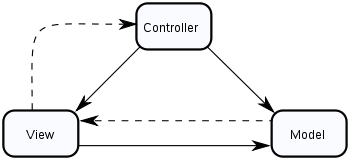
\includegraphics[width=0.5\textwidth]{Images/ModelViewController}
\end{figure}

\begin{itemize}
\item A \emph{model} represents the information of the application and the rules to manipulate that data. In Rails, models are used for managing the rules of interaction with a corresponding database table. In most cases, one table in your database will correspond to one model in your application. Your application logic will be concentrated in the models.
\item A \emph{view} represents the user interface of your application. In Rails, views are often HTML files with embedded Ruby code (which we call erb templates) to perform tasks related to the presentation of the data. Views handle the job of providing data to the web browser or other tool that is used to make requests to your application.
\item \emph{Controllers} provide the “glue” between model and views. In Rails, controllers are responsible for processing the incoming requests from the web browser, interrogating the models for data, and passing the data to the views for presentation.
\end{itemize}

The benefits of using MVC include the isolation of business logic from the user interface.
In addition it becomes easier to keep the code DRY, and 
it makes clear where different types of code belong for easier maintenance.



\section{Convention over Configuration} 
Traditionally, frameworks need multiple configuration files, each with many settings. 
These provide information specific to each project, ranging from URLs to mappings between classes and database tables. 
With the complexity of an application, the size and number of those files grows as well. 
Most of the time, it is very hard to maintain a lot of configurations files. 
Rails was developed to minimize these issues by following the \emph{Convention over Configuration} paradigm.

\emph{Convention over Configuration} aims at simplifying the development without losing the application flexibility. 
It means you do not need to write configuration files in order to have a flexible application. 
This leads to less code and less repetition.
The Rails creator calls this “Intelligent Patterns”. 
If you do not want to configure anything, just follow the conventions and the framework will know what to do.

To better understand \emph{Convention over Configuration}, 
let's see how Rails analyses a URL such as the following:

\begin{rubycode}{URL Example}{lst:rails_url}
  /account/show/1

\end{rubycode}
By default, the framework will split the URL by “/” and following the rest standards, 
we can expect a few things to be true: 

\begin{itemize}
\item \emph{account} – It probably means that a controller called “AccountController” exists in the application. It should be a class that extends the ApplicationController class and handles all kind of actions related with accounts.
\item \emph{show} – The AccountController class should have a show method.
This method will probably interact with a model called Account to fetch the needed data and pass it to a view, 
which will render a nice page showing the account information.
\item \emph{1} – Since we are in the accounts show action, this is the parameter called “id” with the value “1”. 
It means that user want to see information about the account whose id is 1. 
\end{itemize}

Although it is fairly easy to change this behavior (in fact, it is a best practice to change it a little bit) 
without writing one line of code, a Rails application freshly created will expect all those things.
We simply need to create the controller, a view, and have a database, with the correct names and everything will work by itself. 
In many others frameworks, it is necessary to create one or more configuration files, normally XML files.

Another example of \emph{Convention over Configuration} is with respect to the persistence layer 
(which typically deals with a database). 
The only thing you need to do in order to map a Model to its table in the database is 
the code shown in~\ref{lst:rails_product_model}.
\begin{rubycode}{Sample Model file “product.rb”}{lst:rails_product_model}
class Product < ActiveRecord::Base 
end
\end{rubycode}

That is enough for the class to be bound by the framework with a table in the database called Products, and all of its columns will be accessible for use without creating a configuration file to map it. Note as well that you do not need to create getter and setter methods, as they will be there ready to use.
Rails has a concept of pluralize, which means a model Product will have a table Products in the database, or a model Customer will have a table Customers, and so on.



\section{Don’t Repeat Yourself} 
Don’t Repeat Yourself (DRY) is an approach aimed at reducing duplication. 
The philosophy emphasizes that information should not be duplicated, 
because duplicates increase the difficulty of code maintenance, 
decrease clarity, and lead to opportunities for inconsistencies.

DRY is applied quite broadly to include database schemas, 
test plans, the build system, and even documentation. 
When the DRY principle is applied successfully, 
a modification of any single element of a system does not change other logically unrelated elements.
DRY code is created by data transformation, which allows the software developer to avoid copy and paste operations.
DRY code usually makes large software system easier to maintain, 
as long as the data transformations are easy to create and maintain.
DRY is not about just avoiding code duplication, 
but more generally about avoiding multiple and possibly diverging ways to express every piece of knowledge: 
e.g., logic, database schemas, and constants.
If we are always repeating the same code, 
refactoring will be in order to keep your code DRY compliant. 



\section{The Framework Structure} 
Every Rails application follows the same file structure organization. 
This way everything should be in the right spot.

After generating a new Rails application 
(this is achieved by running just the single command line shown in Listing~\ref{lst:new_rails_app} ) 
\begin{rubycode}{Command to create a new rails application}{lst:new_rails_app}
  rails new <name_of_the_appliction>,

\end{rubycode}
a folder looking like the tree in Figure~\ref{fig:rails_file_structure} should be created. 
It is a ready to run web application.

The folder called \emph{app} 
is where the majority of the real code for the new application goes (models, views, controllers, helpers, etc).
The other folders are usually destined to documentation, configuration, third party code, temporary files, etc.

\begin{figure}[h!]
  \caption{Rails Project File Structure}\label{fig:rails_file_structure}
  \centering
  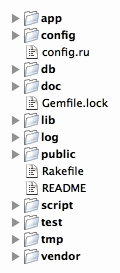
\includegraphics[scale=0.75]{Images/rails_files}
\end{figure}

Rails is a \textsf{meta-framework}\footnote{
  A meta-framework is a framework composed of smaller frameworks.
}, it is composed of the following frameworks:


\subsection{Active Record}
Active Record connects business objects and database tables to create a persistable domain model where logic and data are presented in on wrapping. It’s an implementation of the object-relational mapping (ORM) pattern by the same name as described by Martin Fowler.
Active Record is the base for the models in a Rails application.

It provides database independence, basic CRUD (Create, Read, Update, and Delete) functionality, advanced finding capabilities, and the ability to relate models to one another, among other services.


\subsection{Action Pack} 
Action Pack splits the response to a web request into a controller part (performing the logic) and a view part (rendering a template). This two-step approach is known as an action, which will normally create, read, update, 
or delete some entity defined by a model (often backed by a database) 
before choosing either to render a template or redirecting to another action.

Action Pack implements these actions as public methods on Action Controllers and uses Action Views to implement the template rendering. Action Controllers are then responsible for handling all the action relating to a certain part of an application, 
such as listing, creating, deleting, and updating records.

Action View templates are written using embedded Ruby in tags mingled in with the HTML. 
To avoid cluttering the templates with code, a bunch of help classes provide common behavior for forms, dates, and strings. 
Additionally, it is easy to add specific helpers to keep the separations as the application evolves.


\subsection{Action Mailer}  
Action Mailer is a framework for building e-mail services. You can use Action Mailer to send emails based on flexible templates, or to receive and process incoming email.


\subsection{Active Support} 
Active Support is an extensive collection of utility classes and standard Ruby library extensions that are used in the Rails. 
All these additions have hence been collected in this bundle as a way to gather all that sugar that makes Ruby sweeter. 
For instance, the examples shown previously regarding date and time calculations are part of this bundle.


\section{Rails Community} 
The biggest part of Ruby developers are in fact Rails developers. 
Moreover, Rails is considered the biggest influence on Ruby popularity
(tens of thousands of Rails applications are online).
In addition, Rails developers are also web developers, 
so we can assume that the majority of Ruby and Rails developers also write HTML, Javascript and CSS.
The Ruby and Ruby on Rails community has been growing up in the last few years. 
Programmers from other languages such as Java and .NET are discovering the power of Ruby and how easy it is 
to create web application using Rails.

Ruby and Ruby on Rails community members love conventions and best practices.
It is also common to associate Ruby on Rails with Behaviour Driven Development (BDD) and Agile methodologies.
For instance, a lot of Ruby on Rails book authors speak about automated tests, 
written using domain specific languages (DSLs) such as Cucumber or Rspec. 
This may seem to be an advanced topic, but writing automated tests in Ruby is fairly easy,
and DSLs like Cucumber and Rspec follow the human/natural philosophies of Ruby.

In ~\ref{lst:cucumber}, a simple Cucumber test file shows how readable Cucumber tests can be.

It looks like a use-case, but this is a real automated test. 
By using the power of regular expressions and Ruby dynamic capabilities,
it is possible to parse this Cucumber file and check if the software is valid according to the specification. 

\begin{rubycode}{Cumber feature}{lst:cucumber}
Feature: Search courses
  Potential students should be able to search for courses

  Scenario: Search by topic
    Given there are 34 courses which do not have the topic "math"
    And there are 2 courses LEI, MEI that each have "math" as one of the topics
    When I search for "math"
    Then I should see the following courses:
      | Course code |
      | LEI         |
      | MEI         |
\end{rubycode}

There are a lot of open source projects, frameworks and communities. 
However, as it was shown throughout this chapter, the characteristics of Rails and the various philosophies underlying it
makes this community of great potential to be a starting point to understand the role of best practices, 
their benefits, and how to measure it. 

Later in this document, we will identify which ones are the most relevant Rails best practices,
and discover if the projects that do follow best practices are truly the projects with more success in the community.


  \thispagestyle{empty}
\chapter{Software Metrics}\label{chap:software_metrics}

In this chapter, you will learn the basics of software metrics. 
A brief explanation of quality attributes is given. Furthermore, we stand that, in the context of open source software, maintainability is the most relevant attribute. A few traditional software metrics are listed.


%%--------------------------------------
%% Assessing Open Source Software
\section{Assessing Open Source Software} \label{sec:assessing}
The simplest operation in science and the lowest level of measurement is classification~\cite{kan2002metrics}.

By assessing OSS we mean to sort OSS projects into an
\textsf{ordinal scale}\footnote{Ordinal scale refers to the measurement operations through which the subjects can be compared in order.}
This can be achieved by defining a
\textsf{ranking system}\footnote{
  Ranking system example: to classify a quality attribute, for instance the project documentation, according to its quality with
  five, four, three, two or one star.
} and by placing OSS projects into quality categories with respect to certain quality attributes.
First, we need to find a way of quantifying those OSS quality attributes.

%% Sofware Quality
In software, quality is an abstract concept. It is commonly recognized as lack of "bugs," and meeting the functional requirements.
However, quality can be perceived and interpreted differently based on the actual context, objectives, and interests of each project.
Many software development companies do monitor costumer satisfaction as a quality index.
For instance, IBM ranks their software products in levels of CUPRIMDSO~\cite{kan2002metrics}:
\begin{itemize}
\item Capability/Functionality (refers to the software meeting its functional requirements)
\item Usability (refers to the required effort to learn and operate the software)
\item Performance/Efficiency (refers to the software performance and resource consumption)
\item Reliability (refers to software fault tolerance and recoverability)
\item Instalability/Portability (refers to the required effort to install or transfer the software to another environment)
\item Maintainability (refers to the required effort to modify the software)
\item Documentation/Information (refers to the coverage and accessibility of the software documentation)
\item Service (refers to the company monitoring and service)
\item Overall (refers to an overall classification based on the other attributes)
\end{itemize}
Almost every big software company has similar quality attributes.
ISO/IEC 9126 provides a framework for the evaluation of software quality (The goal is to achieve quality in use, in other words, quality from the user perspective)~\cite{bevan1999quality}
IISO/IEC 912 defines six software quality attributes:
\begin{itemize}
\item Functionality (refers to the software meeting the functional requirements)
\item Reliability (refers to software fault tolerance and recoverability)
\item Usability (refers to the required effort to learn and operate the software)
\item Efficiency (refers to the software performance and resource consumption)
\item Maintainability (refers to the required effort to modify the software)
\item Portability (refers to the required effort to transfer the software to another environment)
\end{itemize}
Quality attributes have interrelationships.
They can be
conflictive\footnote{Conflictive, negative influence, if one attribute is high it makes the other one low.} or
support\footnote{Support, positive influence, if one attribute is high it makes the other one high too.} one another.
For example, the higher the functional complexity of the software, the harder it becomes to achieve maintainability~\cite{kan2002metrics}.

Because of the OSP bazaar style and continuous development process, it is intuitive that the maintainability and documentation attributes
have a big influence on the overall quality and continuous progress of an OSP.
Maintainability and documentation have support relationships
with usability, reliability and availability attributes, but might be conflictive with functionality and performance attributes.

Failure to meet functionality often leads to late changes and increased costs in the development process.
The software industry and researchers have been mostly interested on testing methodologies
that focus on functional requirements and pay little attention to non-functional requirements~\cite{chung2009non}.

There are several challenges and difficulties in assessing non-functional quality attributes for software projects.
For example, security is a non-functional requirement that needs to be addressed in every software project.
Therefore, badly-written software may be functional, but subject to buffer overflow attacks.
Another example is the amount of codebase comments. If the code does not have any comments, it will not affect the functional requirements,
but it is obvious that it will decrease readability and maintainability~\cite{gousios2007software}.

%% SOFTWARE METRICS
\section{Classic Software Metrics}
To classify OSS with regards to a certain quality attribute, we need to find which factors influence it.
Then we need a way to measure that attribute. If we need to make measurements, we need metrics.

Fortunately, there are around two thousand documented software metrics, but there is few information on how those metrics relate to each other.
Most of them simply have different names, but give similar information~\cite{fenton1999software}.
The major challenge is to discover how important the information given by those metrics is, if the calculation effort pays off,
how to interpret their values, and find
\textsf{correlations}\footnote{Correlation is probably the most widely used statistical method to assess relationships among observational data~\cite{kan2002metrics}.}
 to assess the quality attributes of an OSP.


\subsection{Lines of Code}
A line of code is any line of program text that is not a comment or blank line, 
regardless of the number of statements or fragments of statements in the line. 
This specifically includes all lines containing program headers, declarations, and executable and non-executable statements.~\cite{conte1986software}
The lines of code (LOC) metric is anything but simple. 
The major problem comes from the ambiguity of the operational definition: the actual counting.
In the early days of Assembler programming, in which one physical line was the same as one instruction, the LOC definition was clear.
With the availability of high-level languages, the one-to-one correspondence broke down.
Differences between physical lines and instruction statements (or logical lines of code), 
and differences among languages contribute to the huge variations in counting LOC.
For instance, Boehm~\cite{boehm2009software} counts lines as physical lines and includes executable lines, data definitions, and comments. 
Even within the same language, the methods and algorithms used by different counting tools can cause significant differences in the final counts.

Next, the most common variations are described~\cite{jones1986programming}: 
\begin{itemize}
\item Count only executable lines. 
\item Count executable lines plus data definitions. 
\item Count executable lines, data definitions, and comments. 
\item Count executable lines, data definitions, comments, and job control language. 
\item Count lines as physical lines on an input screen. 
\item Count lines as terminated by logical delimiters. 
\end{itemize}


\subsection{Cyclomatic Complexity}
The measurement of cyclomatic complexity~\cite{mccabe1976complexity} was designed to indicate a program's testability and maintainability.
It is the classical graph theory cyclomatic number that indicates the number of regions in a graph.
As applied to software, it directly measures the number of linearly independent paths through a program source code.
Basically, it counts how many different executions a program can have. 
For instance, one "if" statement will double the number of paths. 
Therefore, a high number of control statements (ifs, loops, etc) in a program source code will result in a high cyclomatic complexity. 
As such, it can be used to indicate the effort required to test a program. To determine the paths, the program procedure is represented as a strongly connected graph with unique entry and exit points. The general formula to compute cyclomatic complexity is: 
$$M = V(g) = e - n + 2p$$
where
\begin{itemize}
\item \emph{$V(g)$} is the cyclomatic number of g 
\item \emph{$e$   } is the number of edges 
\item \emph{$n$   } is the number of nodes 
\item \emph{$p$   } is the number of unconnected parts of the graph 
\end{itemize}


\subsection{Fan-In and Fan-Out}
Fan-in and fan-out are perhaps the most common design structure metrics, which are based on the ideas of coupling~\cite{yourdon1979structured}:
\begin{itemize}
\item \emph{Fan-in } is a count of the modules that call a given module
\item \emph{Fan-out} is a count of modules that are called by a given module
\end{itemize}

In general, modules with a large fan-in are relatively small and simple, and are usually located at the lower layers of the design structure.
In contrast, modules that are large and complex are likely to have a small fan-in.
There is also the theory that high fan-outs represent a high number of method calls and thus are undesirable,
while high fan-ins represent a high level of reuse~\cite{wang2007dynamic}.

\subsection{Object-Oriented Metrics}
Classes and methods are the basic constructs of OO technology.
The amount of function provided by an OO software can be estimated based on the number of identified classes and methods or their variants.
Therefore, it is natural that the basic OO metrics are related to classes, methods, and their size.

The pertinent question therefore, is what the optimum value should be for OO metrics. There may not be one correct answer,
but based on his experience in OO software development, Lorenz proposed eleven metrics as OO design metrics called rules of thumb~\cite{lorenz1994object}.
\begin{itemize}
\item \emph{Average Method Size (LOC)}: Should be less than 8 LOC for Smalltalk and 24 LOC for C++
\item \emph{Average Number of Methods per Class}: Should be less than 20. Larger averages indicate too much responsibility in too few classes.
\item \emph{Average Number of Instance Variables per Class}: Should be less than 6. More instance variables indicate that one class is doing more than it should.
\item \emph{Class Hierarchy Nesting Level (Depth of Inheritance Tree, DIT)}: Should be less than 6, starting from the framework classes or the root class.
\item \emph{Number of Class/Class Relationships in Each Subsystem}: Should be relatively high. This item relates to high cohesion of classes in the same subsystem. If one or more classes in a subsystem don't interact with many of the other classes, they might be better placed in another subsystem.
\item \emph{Average Number of Comment Lines (per Method)}: Should be greater than 1.
\end{itemize}




%%%%%%%%%%%%%%%%%%%%%%%%%%%%%%%%%%%%%%%%%%%%
%% AVAILABLE TOOLS
\section{Available Tools}
Tools are intended to make a task easier.
Codebase analysis tools are designed turn the task of analysis and measure source code easier.
Those tools help in the process of finding software flaws and can also serve as aids for assessing the quality of software.

Next a list of some free tools:
\begin{itemize}
\item\textsf{FindBugs} finds "bugs" in Java programs
\item\textsf{FxCop (Microsoft)} analyzes managed code assemblies and reports information about the assemblies
\item\textsf{PMD} scans Java source code and looks for potential code problems
\item\textsf{PreFast} (Microsoft) is a static analysis tool that identifies defects in C/C++ programs
\item\textsf{RATS} (Fortify) scans C, C++, Perl, PHP and Python source code for security problems like buffer overflows and Time Of Check, Time Of Use race conditions
\item\textsf{SWAAT} simplistic tool for Java, JSP, ASP .Net, and PHP
\item\textsf{Flawfinder} scans C and C++
\item\textsf{Saikuro} is a Ruby cyclomatic complexity analyzer.
\item\textsf{Reek} is a tool that examines Ruby classes, modules, methods and reports any code smells it finds.
\item\textsf{Rails best practices} is another tool that examines Ruby classes, modules, methods and reports any code smells it finds.




\end{itemize}

Tools like the ones listed above analyze code without executing it and point out what they consider to be potential weaknesses.
The most typical example of what those tools can find is most likely calls to the emph{gets} function in
the C programming language. This function is inherently insecure and can lead to buffer
overflows. Specially crafted user input values can, for instance, allow an attacker to access
or modify confidential data or even take control of any computer executing that piece of
software.

Because these tools need to "understand" the code being analyzed, they are necessarily very language specific.
Furthermore, when analyzing a large amount of software projects, for instance GitHub projects,
it is of great importance to have a previous knowledge of what kinds of projects  are going to be found (programming languages, frameworks, and other attributes).
This way tools can be adapted to get better results. 


  \thispagestyle{empty}
\chapter{Best Practices}\label{chap:best_practices}

Best practices are not rules, they are standards followed by a specific community.
Something that most people agrees with, although it might not be scientifically proven,
it seems to be the best way of handling a problem.

In this chapter we will understand how important best practices are for open source communities, 
how they give meaning to traditional software metrics
and identify some examples of best practices from the ruby community.


\section{Best Practices in Open Source Software Projects} \label{sec:best_practices_ossp}
Open source communities have a tendency to create \emph{coding rules},
i.e., \emph{principles governing the conduct of programmers and serving as a basis of measure or judgment}. 
It is a natural and evolutive process for people surviving in an open space.
We can call these natural rules: \emph{best practices}.

Best practices are  methods thought as being the  best way for achieving something;
they are spread through the community and everybody does it that way.
It is obvious that when a developer follows well established principles and best practices, 
the project maintainability is increased.
Consequently, project new comers will find it easier to understand the project code~\cite{dromey2002model}.
But there is more than that, following best practices discourage:
\begin{itemize}
\item Poor performance (due to bad patterns)
\item Poor error checking (defensive programming)
\item Inconsistent exception handling / Maintainability (long-term quality)
\end{itemize}

To attain the same benefits, companies define standards, this is, something considered by an authority 
as a basis of comparison and a normal requirement for quality;
by other words, an approved behavior model for their workers.
However, these principles are defined by the few people on top and then spread down on the pyramid.
Many times, those rules are not well thought by the project leaders and that can block the progress.

In the other way around, the apparent chaos of open source also requires some rules,
but contrary to the companies coding standards, which work in a top down way,
best practices happen in a bottom up and distributive mode,
everybody can try different ways of doing things,
but the ones with better results are most likely to be copied.

A simple metaphor exposes the difference:
\begin{quote}\emph{
  Companies use traffic lights where open source communities use roundabouts.
}\end{quote}

Both, the strict company standards (traffic lights) and the OSP best practices (roundabouts) are ways to regulate intersections.
The result of traffic lights is  easier to predict, however that regulation  system does not depend much on the drivers skills;
because it is so restrictive it will happen often to find a driver stooped alone
at the crossroads waiting for a green light, losing precious time.
On the other hand, the roundabout system is a less restricted system and relies much more on the quality of the drivers,
but it open the possibility to a much more efficient way to avoid a traffic jam.

There is little work done concerned with measuring coding best practices by automatic analyzing source code.
A plausible explanation for that is the fact that best practices are not a set of immutable rules,
they are a continuous evolution and improvement of development methodologies.
Communities are constantly creating rules and best practices, even without noticing it.
It is not possible to write down a list of best practices without some ambiguities.

At first glance, best practices metrics seam to be for classic metrics as natural as medicine is for science.
But, it is not the case.
In fact, classic metrics, on their own, do not give much information about a project.
In many cases, best practices can be the key to understand what should be the optimum value for a classic metric,
for instance, to determine \emph{how many lines of code should a ruby method have}.

Of course, those questions are subjective.
However, by analyzing renowned projects, developers opinions and so on, it is possible to find out a best practice
that gives a plausible answer to the search for the \emph{most favorable value}.

In addition, it is possible to use known source code metrics and, by analyzing their values, 
to find new correlations that might give hints about weather some methodological approaches were 
taken into account during the project development process.

We believe that best practices can give a meaning to metrics.

\section{Identifying Best Practices} \label{sec:identifying_best_practices}
We understood that software projects can benefit a lot from using best practices.
However, what is a best practice after all?
The truth is that everything can be a best practice, for example:
the use of two spaces to indent code and no tabs; 
writing unit tests for your code;
the way files are organized inside a project; etc.

Some of those things might look like a matter of taste,
but the truth is that every worthy ruby developer uses two spaces to indent code.
This is the standard for the ruby community. 
Other communities, for instance JavaScript programers, prefer 4 spaces
and in the Java world 8 spaces is considered the considered a good choice.

It is important to notice,
that we can find virtually no ruby programmer using a different indentation, 
but we can find Java communities advocating different indentations.
This fact shows that the ruby community agrees that 2 spaces is a the best option and
can be considered a best practice.
In contrast, we can not be completely sure about the 8 spaces for Java,
since there is also a lot of developers advocating 4 spaces and also a good number using tabs instead.
The Java community is divide, it almost possible to identify sub communities defending 
different answers for the same questions. 
It might be possible to identify conventions in those smaller communities, 
but it will be harder to do it for the bigger community.

To consider this conventions as a best practice, it is important to understand if that
conventions are strong through the community in question. 
Because of that, it is obvious that the first step before finding best practices is to identify the community:
are we trying to find best practices for ruby programers general? for all programers in general? 
for the programers working in a specific company or project?

In smaller communities, it might be easier to achieve agreement and
consequently find best practices.
However, best practices created and followed by a small groups,
are less likely to be considered strong best practices compared to 
best practices followed by the developers working on the top 10 open source projects.

It is clear that best practices are specific to a certain community, 
so, after correctly choosing a community, to find identify best practices we need
to find out what patterns are used by its members, 
and to prove that they are real best practices that should be followed, 
it is important to prove that some benefit comes from using it.

The most obvious benefit from using it,
is that the project maintainability is increased,
for example: people in the community might be expecting to find the code indented with two spaces or 
methods named in camelcase, constants in upcase, etc.

Supposedly using two or more spaces does not affect directly the code quality (other than maintainability), 
but it is reasonable to infer that a developer is new to ruby if he does not know it.
In other words, following, or not, best practices has a relation with the developer knowledge and experience,
and the developer experience is likely to be related with the code quality produced.

Of course, best practices are not only related to naming,
they can also be patterns for solving certain problems, working methodologies, etc.
In those cases, they might be directly related to other quality attributes like performance and so on.

In the end, it seems plausible to believe that there is a correlation between this two variables.
The quantity of best practices followed and the overall quality of the project. 

Later in this document, this relation between these variables relation is proved.


\section{Best Practices Examples} \label{sec:best_practices_examples}
In this section, different best practices categories are listed.

These are best practices for the ruby community.

Best practices related to code formatting:
\begin{itemize}
\item \emph{Use two spaces to indent code and no tabs}, every worthy ruby developer do it that way.
\item \emph{Remove trailing whitespace}, trailing whitespace makes noises in version control systems.
\end{itemize}

Related to syntax:
\begin{itemize}
\item \emph{Avoid return where not required}.
\item \emph{Suppress superfluous parentheses}, when calling methods, 
but keep them when calling \"functions\" (when you use the return value in the same line).
\end{itemize}

Related to naming:
\begin{itemize}
\item \emph{Use snake\_case for methods}.
\item \emph{Other method naming conventions}: Use map over collect, find over detect, find\_all over select, size over length.
\end{itemize}

Specific to a framework (Ruby on Rails in for the following examples):
\begin{itemize}
\item \emph{Law of Demeter}, A model should only talk to its immediate association.
\item \emph{Move code into controller}, according to MVC architecture, there should not be logic codes in view.
\item \emph{Isolate seed data}, do not insert seed data during migrations, a 
rake task\footnote{ 
  Rakefiles work in similar way to Makefiles but are written in ruby. It is a simple way to write code to automate repetitive tasks. 
} can be used instead.
\item \emph{Do not use default route}, When using a RESTful design. The default RoR routes can cause a security problems.
\item \emph{Replace Complex Creation with Factory Method}, Sometimes you will build a complex model with params, current\_user and other logics in controller, but it makes your controller too big, you should move them into model with a factory method.
\end{itemize}




\section{Ruby on Rails Best Practices} \label{sec:ror_best_practives}

Ruby and Ruby on Rails community members are, in general, known has been addicted to best practices.
In reality, many of those best practices are studied development methodologies.
It is common to associate Ruby on Rails with Behaviour Driven Development (BDD) and Agile methodologies.
And, most ruby developers, even language new comers, are worried about following Rails philosophies and best practices.
The majority of Ruby on Rails book authors speak about convention over configuration,
those conventions can be be seen as best practices too.

Because of all this, the Rails community has great potential to be a starting point to understand the role of best practices, 
what benefits come from using it and how to measure best practices.

The first step is to define the community: Rails developers. 
After that, we need to find procedures or methodologies that most of people, in the community, agrees to consider it as best practice.
The simplest way is to ask people in the community. 
In fact, there was already some work done here.
The web site
\textsf{Rails Best Practices}\footnote{\url{http://www.rails-bestpractices.com/} is a web site created by Richard Huang,
it was inspired by Wen-Tien Chang talk given at Kungfu RailsConf 2009 in Shanghai. Slides can be found here
\url{http://www.slideshare.net/ihower/rails-best-practices}.},
works in similar way to a web forum and its objective is to engage developers to discuss which practices
should be considered best practices to follow, when building a Rails web application.
At Rails Best Practices Web Site, every Rails developer can suggest new best practices,
improve and comment suggested best practices and vote whether he considers it a best practice or not.

After deciding that some \emph{procedure} is a \emph{best practice},
it would be handy to find a way to automatically verify whether 
that practice is being followed by the developers of a given project.
With that in mind, an open source ruby 
\textsf{gem}\footnote{
  Ruby Libraries are called gems. Ruby gems can be easily managed using rubygems 
  (rubygems is for Ruby as aptitude is for Debian or cpan for perl).
}, 
called rails\_best\_practices, was created (by the authors of Rails best practices web site) 
based on the most voted best practices. 
After installing the gem, it is possible to run it against any Rails project.
and it will automatically produce a report that shows where,
in the source code, a project is failing to obey to consensual best practices.
It is important to notice that the rails\_best\_practices gem does not say if a project is following best practices,
it does the opposite, shows where the project is failing.

At the moment of writing, this gem can check for 33 different best practices from more then 70 described in the web site.
We did a few commits to this gem source code, to improve and correct some bugs, 
everybody is welcome to do it and to help with the writing of more best practices failing detectors.

\subsection{Best Practices Considered}\label{subsec:second_study}



\subsubsection{Remove Tab}
  Make sure there are no tabs in files.
 
  % See the best practice details here \url{http://rails-bestpractices.com/posts/81-remove-tab}
   
\subsubsection{Remove Trailing Whitespace }  
  Make sure there are no trailing whitespace in codes.
 
  % See the best practice details here \url{http://rails-bestpractices.com/posts/60-remove-trailing-whitespace}
   
\subsubsection{Add Model Virtual Attribute}
  Make sure to add a model virual attribute to simplify model creation.
 
  % See the best practice details here \url{http://rails-bestpractices.com/posts/4-add-model-virtual-attribute}
       
\subsubsection{Always Add Db Index}
  Review db/schema.rb file to make sure every reference key has a database index.
 
  % See the best practice details here \url{http://rails-bestpractices.com/posts/21-always-add-db-index}
       
\subsubsection{Dry Bundler In Capistrano}
  Review config/deploy.rb file to make sure using the bundler's capistrano recipe.
 
  % See the best practice details here \url{http://rails-bestpractices.com/posts/51-dry-bundler-in-capistrano}
   
\subsubsection{Isolate Seed Data }
  Make sure not to insert data in migration, move them to seed file.
 
  % See the best practice details here \url{http://rails-bestpractices.com/posts/20-isolating-seed-data.}
   
\subsubsection{Keep Finders On Their Own Model}
  Review model files to ake sure finders are on their own model.
 
  % See the best practice details here \url{http://rails-bestpractices.com/posts/13-keep-finders-on-their-own-model.}
   
\subsubsection{Law Of Demeter }
  Review to make sure not to avoid the law of demeter.
 
  % See the best practice details here \url{http://rails-bestpractices.com/posts/15-the-law-of-demeter.}
   
\subsubsection{Move Code Into Controller}
  Review a view file to make sure there is no finder, finder should be moved to controller.
 
  % See the best practice details here \url{http://rails-bestpractices.com/posts/24-move-code-into-controller.}
   
\subsubsection{Move Code Into Helper }
  Review a view file to make sure there is no complex options\_for\_select message call.
 
  % See the best practice details here \url{http://rails-bestpractices.com/posts/26-move-code-into-helper.}
   
\subsubsection{Move Code Into Model }
  Review a view file to make sure there is no complex logic call for model.
 
  % See the best practice details here \url{http://rails-bestpractices.com/posts/25-move-code-into-model.}
     
\subsubsection{Move Finder To Named Scope }
  Review a controller file to make sure there are no complex finder.
 
  % See the best practice details here \url{http://rails-bestpractices.com/posts/1-move-finder-to-named_scope.}
   
\subsubsection{Move Model Logic Into Model}
  Review a controller file to make sure that complex model logic should not exist in controller, should be moved into a model.
 
  % See the best practice details here \url{http://rails-bestpractices.com/posts/7-move-model-logic-into-the-model.}
   
\subsubsection{Needless Deep Nesting}
  Review config/routes.rb file to make sure not to use too deep nesting routes.
 
  % See the best practice details here \url{http://rails-bestpractices.com/posts/11-needless-deep-nesting.}
   
\subsubsection{Not Use Default Route}
  Review config/routes file to make sure not use default route that rails generated.
 
  % See the best practice details here \url{http://rails-bestpractices.com/posts/12-not-use-default-route-if-you-use-restful-design}
   
\subsubsection{Not Use Time Ago In Words}
  Review view and helper files to make sure not use time\_ago\_in\_words or distance\_of\_time\_in\_words\_to\_now.
 
  % See the best practice details here \url{http://rails-bestpractices.com/posts/105-not-use-time_ago_in_words.}
   
\subsubsection{Overuse Route Customizations}
  Review config/routes.rb file to make sure there are no overuse route customizations.
 
  % See the best practice details here \url{http://rails-bestpractices.com/posts/10-overuse-route-customizations.}
   
\subsubsection{Protect Mass Assignment}
  Review model files to make sure to use attr\_accessible or attr\_protected to protect mass assignment.
 
  See the best practices details here \url{http://rails-bestpractices.com/posts/148-protect-mass-assignment.}
   
\subsubsection{Remove Empty Helpers Review}
  Review a helper file to make sure it is not an empty moduel.
 
  % See the best practice details here \url{http://rails-bestpractices.com/posts/72-remove-empty-helpers.}
   
\subsubsection{Remove Unused Methods In Controllers}
  Find out unused methods in controllers.
   
\subsubsection{Remove Unused Methods In Helpers}
  Find out unused methods in helpers.
       
\subsubsection{Remove Unused Methods In Models}
  Find out unused methods in models.
   
\subsubsection{Replace Complex Creation With Factory Method}
  Review a controller file to make sure that complex model creation should not exist in controller, should be replaced with factory method.
 
  % See the best practice details here \url{http://rails-bestpractices.com/posts/6-replace-complex-creation-with-factory-method.}
   
\subsubsection{Replace Instance Variable With Local Variable}
  Review a partail view file to make sure there is no instance variable.
 
  % See the best practice details here \url{http://rails-bestpractices.com/posts/27-replace-instance-variable-with-local-variable.}
   
\subsubsection{Restrict Auto Generated Routes}
  Review a route file to make sure all auto-generated routes have corresponding actions in controller.
 
  % See the best practice details here \url{http://rails-bestpractices.com/posts/86-restrict-auto-generated-routes}
   
\subsubsection{Simplify Render In Controllers}
  Review a controller file to make sure using simplified syntax for render.
 
  % See the best practice details here \url{http://rails-bestpractices.com/posts/62-simplify-render-in-controllers.}
   
\subsubsection{Simplify Render In Views}
  Review a view file to make sure using simplified syntax for render.
 
  % See the best practice details here \url{http://rails-bestpractices.com/posts/61-simplify-render-in-views.}
   
\subsubsection{Use Before Filter}
  Review a controller file to make sure to use before\_filter to remove duplicated first code line in different action.
 
  % See the best practice detailed here \url{http://rails-bestpractices.com/posts/22-use-before_filter.}
   
\subsubsection{Use Model Association}
  review a controller file to make sure to use model association instead of foreign key id assignment.
 
  % See the best practice details here \url{http://rails-bestpractices.com/posts/2-use-model-association.}
   
\subsubsection{Use Multipart Alternative As Content Type Of Email}
  Make sure to use multipart/alternative as content\_type of email.
 
  % See the best practice details here \url{http://rails-bestpractices.com/posts/41-use-multipart-alternative-as-content\_type-of-email.}
   
\subsubsection{Use Observer}
  Make sure to use observer (sorry we only check the mailer deliver now).
 
  % See the best practice details here \url{http://rails-bestpractices.com/posts/19-use-observer.}
   
\subsubsection{Use Query Attribute}
  Make sure to use query attribute instead of nil?, blank? and present?.
 
  % See the best practice details here \url{http://rails-bestpractices.com/posts/56-use-query-attribute.}
   
\subsubsection{Use Say With Time In Migrations}
  Review a migration file to make sure to use say or say\_with\_time for customized data changes to produce a more readable output.
 
  % See the best practice details here \url{http://rails-bestpractices.com/posts/46-use-say-and-say\_with\_time-in-migrations-to-make-a-useful-migration-log.}
   
\subsubsection{Use Scope Access}
  Review a controller to make sure to use scope access instead of manually checking current\_user and redirect.
 
  % See the best practice details here \url{http://rails-bestpractices.com/posts/3-use-scope-access.}



  \thispagestyle{empty}
\chapter{Assessing Ruby on Rails Projects}\label{chap:assissing_ror}


%%--------------------------------------
%% ASSESSING RUBY ON RAILS PROJECTS
\section{Assessing Ruby on Rails Projects} \label{sec:assessing_ror}
After deciding that some \emph{procedure} is a \emph{best practice},
it would be handy to find a way to automatically verify whether that practice is being followed by
the developers of a given project.
With that in mind, an open source ruby gem was created (by the authors of Rails best practices web site) 
with the objective of automatically producing a report that shows where,
in the source code,  a project is failing to obey to consensual practices.
At the moment of writing, this gem can check for 28 kinds of best practices (from the 70 described in that web site).

However, one of the first things that we have noticed when we have applied this gem to OSS projects,
is that the biggest and most renown projects have much more errors than the smaller and unknown projects.
This nonsense has a simple  interpretation.
%The majority of RoR projects found in github are simple projects, in most cases, developed by a single user.
Small projects (like the majority of RoR projects found in github) are simple software packages,  often 
developed by a single user.
These applications are so simple that many times the code is almost entirely created by RoR code generators.
Usually, when code is not written by humans, it has few mistakes concerning those recommendations.

\subsection{First Study}\label{subsec:first_study}
Having taken the above into account, we decided to run the rails best practices gem on similar RoR (Ruby on Rails) projects.
Seven \emph{time tracking} or \emph{project management} open source systems were chosen.
After running the gem and counting
\textsf{not best practices (NBPs)}\footnote{In fact, Rails best practices gem does not find best practices in the source code.
  It does the opposite, it discovers when the code is not written according to a best practice, in other words, 
  it identifies bad practices (similar to the detection of code smells).
  We decided to name those occurrences NBP.
}
occurrences, the following results were obtained:

\begin{table}[H]
\begin{center}{\scriptsize
  \begin{threeparttable}
  \begin{tabular}{|l||c|c|c|c|c|c|c|} \hline
  \multicolumn{8}{|c|}{Rails Best Practices Results} \\ \hline
  \textbf{Best Practice}& \textbf{A}& \textbf{B}& \textbf{C}&  \textbf{D}& \textbf{F}& \textbf{G}& \textbf{H} \\\hline\hline
  \emph{\tnote{a}Add model virtual attribute           }              &   -  &   2  &   7  &   - &   - &   5 &   4  \\ \hline
  \emph{Always add db index                   }              &   -  &   -  &   -  &  43 &   - &   - &  51  \\ \hline
  \emph{Isolate seed data                     }              &   -  &   -  &   -  &   - &   - &  79 &  17  \\ \hline
  \emph{Law of demeter                        }              &  20  &  38  &  45  &   6 &  30 & 164 &  85  \\ \hline
  \emph{Move code into controller             }              &   -  &   -  &   -  &   - &   2 &   - &   4  \\ \hline
  \emph{Move code into model                  }              &   -  &  26  &   -  &   7 &   1 &   3 &  19  \\ \hline
  \emph{Move model logic into model           }              &   -  &   -  &  76  &  11 &  11 &  98 & 100  \\ \hline
  \emph{Move finder to named\_scope           }              &   -  &   4  &   9  &   2 &   4 &  25 &   -  \\ \hline
  \emph{Needless deep nesting                 }              &   -  &   -  &   -  &   1 &   - &   - &   -  \\ \hline
  \emph{Not use default root                  }              &   -  &   1  &   1  &   - &   1 &   1 &   1  \\ \hline
  \emph{Notes  use query attribute            }              &   -  &   2  &   -  &   - &   - &   - &   -  \\ \hline
  \emph{Overuse route customizations          }              &   -  &   -  &   2  &   4 &   - &   2 &   2  \\ \hline
  \emph{Remove trailing whitespace            }              &  68  &  57  & 126  & 110 & 330 & 316 & 100  \\ \hline
  \emph{Use factory method                    }              &   -  &  15  &   9  &   5 &   1 &   8 &  19  \\ \hline
  \emph{Replace instance var with local var   }              &  13  &   -  &  70  & 239 & 142 &  31 & 100  \\ \hline
  \emph{Use before\_filter                    }              &   -  &   7  &   9  &   8 &   8 &  19 &  23  \\ \hline
  \emph{Wrong email content\_type             }              &   -  &   3  &   -  &   - &   - &   - &   -  \\ \hline
  \emph{Use query attribute                   }              &   -  &   -  &  11  &   5 &   8 &  29 &   6  \\ \hline
  \emph{Use say with time in migrations       }              &   -  &   -  &  24  &   - &  10 &  23 &  56  \\ \hline
  \emph{Use scopes access                     }              &   -  &   -  &   -  &   - &   - &   - &  04  \\ \hline
  \emph{User model association                }              &   -  &   -  &  12  &   9 &   - &   1 &  21  \\ \hline
  \emph{Keep finders on their own model       }              &   8  &   4  &   1  &   - &  11 &   - &   -  \\ \hline
  \emph{Total                                 }              & 109  & 156  & 402  & 450 & 559 & 834 & 864  \\ \hline
  \end{tabular}
  \begin{tablenotes}
    \item \emph{A:} Rubytime
    , \emph{B:} Notes
    , \emph{C:} Tracks
    , \emph{D:} Handy Ant
    , \emph{F:} Retrospectiva
    , \emph{G:} Redmine
    , \emph{H:} Clockingit
    \item Figures shown represent the number of times a project do not follow a best practice; is expected that \emph{smaller the number, better the project}.
  \end{tablenotes}
  \end{threeparttable}
}
\end{center}
\caption{Results obtained by running the \emph{best practices analyzer gem} on the 7 Open Source Projects chosen (data produced on April, 2011).}
\end{table}

Rubytime seems to have the best results and Clockingit the worst. 
The fact is that very good user reviews can be found about Rubytime.
However, Tracks obtained an unexpected high score, since it has been very sparsely maintained 
(old code has higher probability of not following the current best practices).
As explained before, those values are not really measuring if a project follows best practices 
but instead measuring when it fails.
This should also be taken into consideration. 

The most evident problem here is that best practices are not being weighted and neither the size of the project considered.
For instance, if the developers have the habit of leaving trailing white spaces, 
the occurrences of this will obviously be related to the size of the project.
On the other hand, it is a best practice to remove the default route generated by rails, 
independently of the project size this is true or false, there is no way to leave the route two times. 
So, if developers do not take into account those two best practices, when the project grows, 
the number of trailing spaces will increase and the results will show more NBPs, 
but the other one will always be only one NBP.  
Because of that we can get twisted results.

To avoid this, the projects were sized.
The size attribute is based on the quantity of models and controllers in the project.
After that, we divided the values previously obtained  by the project size.
By doing that, a new set of results emerge.

\begin{table}[H]
\begin{center}
{\scriptsize
\begin{threeparttable}
\begin{tabular}{|l||c|c|c|c|c|c|c|} \hline
\multicolumn{8}{|c|}{Rails Best Practices Results} \\ \hline
\textbf{Best Practice}& \textbf{A}& \textbf{B}& \textbf{C}&  \textbf{D}& \textbf{F}& \textbf{G}& \textbf{H} \\\hline\hline
\emph{Total                                           }              & 109  & 156  & 402  & 450 & 559 & 834 & 864  \\ \hline
\emph{Total Without Trailing Whitespace               }              &  41  &  99  & 276  & 340 & 229 & 518 & 764  \\ \hline
\emph{Project Size                                    }              &  12  &  11  &  11  &  29 &  26 &  58 &  31  \\ \hline
\emph{Total / Project Size                            }              &   9  &  14  &  37  &  16 &  23 &  15 &  28  \\ \hline
\emph{Total Without Trailing Whitespace / Project Size}              &   3  &   9  &  25  &  12 &   9 &   9 &  25  \\ \hline
\end{tabular}
\begin{tablenotes}
  \item \emph{A:} Rubytime.
  , \emph{B:} Notes
  , \emph{C:} Tracks
  , \emph{D:} Handy Ant
  , \emph{F:} Retrospectiva
  , \emph{G:} Redmine
  , \emph{H:} Clockingit
\end{tablenotes}
\end{threeparttable}
}
\end{center}
\caption{Results obtained by running the \emph{best practices analyzer gem} on the 7 Open Source Projects chosen, after normalization (data produced on April, 2011).}
\end{table}

Those results are much more likely to be helpful in terms of understanding if a project is or is not following 
best practices.
The numbers reflect both the community reviews and our own estimates much more.


\subsection{Second Study}\label{subsec:second_study}
After the first study reported above, we felt that it was time to make a bigger one;
we should repeat the experiment over a larger sample. 
In addition, there was the need to define an objective quality metric to compare the metrics results with.
As a second target for this new phase, it was decide to find an objective quality rate (a reputation ranking) for each project in the sample, 
to be possible to compare with the results computed for the best practices metrics.

For the second study, we selected 40 Ruby on Rails projects hosted in github and
decided to consider the number of 
\textsf{followers}\footnote{Number of users that want to receive notifications about the project.} and
\textsf{forks}\footnote{Number of people that forked the project. This means that either they want to contribute to the project or create a derived project}, 
that each project has on github, 
as a \emph{project reputation} metric. 

The objective was to prove that a negative correlation exists, between the NBPs of a project and its followers and forks. 

The previous study has shown us the need to apply different weights to each NBP. 
By diving the NBPs by the project size, in the first study, seemed like we got better results.
However, not all NBPs depend on the project size. 
Therefore, we altered the rails best practices gem to make it possible to know how much project files were analyzed 
by each rails best practice checker.

Basically, after collecting the GitHub URLs for each project, we followed the next steps:
\begin{itemize}
\item \emph{Retrieve GitHub information}, in this step we get the followers and forks(and more info that might be used in further analyses).
\item \emph{Download the project repository}.
\item \emph{Run rails best practices gems}, at this point, we get the non weighted NBPs and files given by each one of the 29 checkers.
\item \emph{Calculate the Weighted Global NBPs}, the evaluation algorithm consists in dividing the value returned by each NBP checker  by the number of files checked and, then sum it.
\end{itemize}

Next, an excerpt of the obtained table is shown:
\begin{table}[H]
\begin{center}
{\scriptsize
\begin{threeparttable}
\begin{tabular}{|l||c|c|c|c|c|c|c|c|c|c|c|} \hline
\multicolumn{12}{|c|}{Rails Best Practices Results} \\ \hline
Projects & \textbf{Forks}         & \textbf{Watchers} & 
C1       & C1 F.                  & \textbf{W. C1} & 
C2       & C2 F.                  & \textbf{W.       C1} & 
...      & T. NBPs                & \textbf{W.  T. NBPs} \\\hline\hline
\emph{Rails Admin } & 30 & 2478 &  0 & 141 & \textbf{  0 }&  0 &  37 & \textbf{ 0} & ...&  50 & \textbf{ 739}  \\ \hline
\emph{Rubytime    } & 12 &   82 & 24 & 161 & \textbf{149 }&  0 & 134 & \textbf{ 0} & ...& 146 & \textbf{1334}  \\ \hline
\emph{Redmine     } & 30 & 1781 & 49 & 996 & \textbf{ 49 }&  1 & 362 & \textbf{ 2} & ...& 884 & \textbf{1402}  \\ \hline
\emph{BrowserCMS  } & 30 &  784 & 11 & 234 & \textbf{ 47 }&  0 & 216 & \textbf{ 0} & ...& 268 & \textbf{1510}  \\ \hline
\emph{Tracks      } & 17 &   87 & 46 & 842 & \textbf{ 54 }& 15 & 271 & \textbf{55} & ...& 569 & \textbf{2810}  \\ \hline
\emph{...}&...&...&...&...&...&...&...&...&...&...&...\\ \hline
\end{tabular} 

\begin{tablenotes}
  \item{ \emph{C(x): }} The rails best practices gem has 29 checkers(when this study was carried), each one tries to find occurrences of a different nbp in the project. 
  \item{\emph{C(x) Files: }} The number of files in the project, where it tried to find nbps (for instance, some checkers may only be concerned with html files, some other checker nbps my only occur in model files, etc)
  \item{\emph{W. C(x): }} Weighted C(x) = C(X) / C(x)Files * 1000 (A really small number is added to each variable to avoid divisions by zero).
\end{tablenotes}
\end{threeparttable}
}
\end{center}
\caption{Results obtained by running the \emph{best practices analyzer gem} on the 40 Open Source Projects chosen, from GitHub (data produced on April, 2011). The full table can be found at www.bestpracticesstudy.gorgeouscode.com}
\end{table}

\subsection{Results}\label{subsec:results}
After building a table containing the results for the 40 projects, we easily found correlations between columns.
We discovered that the average correlation index, for the weighted C(x) columns, is -0.2. Only three of the weighted C(x) columns do not have negative correlation. This is quite good, considering the fact that there is an explanation for it. 
Those three checkers (without negative correlation) aimed at finding  NBPs that almost non of the projects were committing, 
so there is no correlation.


The most important results are in the next table:
\begin{table}[H]
\begin{center}
{\scriptsize
\begin{threeparttable}
\begin{tabular}{|l||c|c|} \hline
\multicolumn{3}{|c|}{Correlations} \\ \hline
                       & \textbf{Total NBPs}  & \textbf{Total Weighted NBPs}  \\ \hline\hline
\emph{Forks         }  & 0.14                 & -0.53                       \\ \hline
\emph{Watchers      }  & 0.07                 & -0.40                       \\ \hline
\end{tabular}
\end{threeparttable}
}
\end{center}
\caption{ The full table can be found at www.bestpracticesstudy.gorgeouscode.com}
\end{table}

These correlation indexes show that if we just count the nbps there is no relation between them and the number of forks and watchers. Nevertheless, the Weighted NBPs have a quite perceptible negative correlation both with watchers and forks. 

Observing that Table, it is possible to notice that the forks correlation is bigger. 
We believe that if it happens, it is because forking a project shows intensions of digging into the code and, 
of course, it easier to understand others code when it follows good practices.

As future work, we are considering more correlations with other variables that are already available, but we haven't used yet. The most relevant ones: the number of commiters, starting date of the project, last commit data, and total number of commits. We believe that those variables can strongly be related with the forks, watchers and of course, in the end, the quality of the project.


  \thispagestyle{empty}
\chapter{Conclusion}\label{chap:conclusion}


As it was said in the beginning of this document, thousands of open source software packages can be found online and 
freely downloaded in platforms like GitHub,
the web-based hosting service for projects using the Git revision control system that 
hosts more than 1 million open source projects.

Throughout this study the need for assessing the quality of these open source software projects became clear.
Maintainability turned out to be a crucial attribute in assessing their quality, 
obviously because of the community-driven orientation of these types of projects, 
described in chapter \ref{chap:open_source}. 
However, this statement does not mean that maintainability is not also a quality attribute of great importance
for closed source software projects as well. 
In fact, most standards, studies and tools within the field of measuring the quality of software projects 
were conducted by private companies with the purpose of improving and assuring the quality of their projects,
which were usually closed source software projects. This idea together with the concepts of software quality and 
quality attributes were explored in chapter \ref{chap:software_metrics}.

Few people have the ability to quickly assess the quality of a project by looking at source code. 
An application, able to perform automatic analysis of software projects and to generate a high-level overview of the code,
is beneficial for assessing the quality of general software projects, independent of whether the license is open source.

Nevertheless, open source and closed source usually end up having a different development processes, and 
because of this they should obviously be analyzed in different ways.
In the open source world there are no strict development rules; 
however, as time goes by and projects get bigger, something similar to rules
or standard behaviors start to emerge in an spontaneous way, called best practices.This topic was discussed in chapter \ref{chap:best_practices}.
There is the belief that by following these best practices, better results will be achieved.

In fact, the existence of common guidelines in software projects intuitively seems to be a potenciator of their 
maintainability to every developer.
But just like popular sayings, their value is ambiguous if there is no scientific proof and 
its application could be considered a matter of taste.

However, we strongly believe that best pratices hold an extremely important value.
Best practices are not rigid as standards, which means that their usage is also more flexible.
Despite this, our belief since the beginning of this investigation is that if 
a project follows best practices, it has a higher probability of being a better project when it comes to quality standards.
Following this idea we focused our research towards proving the existence of
a correlation between the quality of the GitHub open source projects and the amount of best practices followed,
as explained in detail in chapter \ref{chap:assissing_ror}.

Initially, when we first started to elaborate this work it seemed like there was no work done 
concerning the measurement of best practices by automatic source code analysis.
As a good surprise and back-up for the ideas described in this document, simultaneous with this research, 
several projects appeared on the scene based on similar ideas and concepts.

In the particular context of Ruby Community, we found that some efforts have already been made in this exact direction,
defining best practices and creating scripts to automatically analyze the source code.
A project called Rails Best Practices, started by Richard Huang, managed to put into practice some of our initial ideas of defining best practices with 
the help of the Rails developers' input and opinions, and even started to create code analyzers to detect whether a project is following them.
The aforementioned project is described in chapter \ref{chap:best_practices}.

However, like most of the reports generated by the existent source code analyzers,
the Rails best practices gem implementation is only spotting the occurrence of bad smells:
not really identifying the best practices, but instead those that are not best practices. 
In chapter \ref{chap:assissing_ror} we named this concept concept of NBPs.
This way it is possible to verify whether a best practice is not being followed, 
since most of the time it is easier to identify incorrection instead of correction.
This turns out to be a clever idea.
These NBP reports are helpful, although not enough, but is a fact that allows the improvement of rails projects.
There existed the need to interpret those results to end up with a high level quality statement.
It was expected that by analyzing a massive amount of open source projects, it would be possible to start understanding
the meaning of the values given by simple metrics,
and thus to judge the impact of these numbers in the quality of the project. 
Consequently, we would find new ways to assess the quality, which is closely related to the level of maintainability, of an open source project.
The final objective was to create a new higher-level metric capable of quantifying the best practices followed by a given project; something as simple as "from 1 to 5, this project has 4 stars in terms of best practices".

To achieve this we started looking for Rails projects hosted in GitHub, 
applying the different metrics and running the NBP checkers, and gathering all this information.
As it was said before, by itself those values are useless; yet
by comparing projects, it was possible to start understanding how to interpret those values.
For instance, obvious things like considering the \emph{size of the project}
(it is intuitive that a project with 10 lines of code and 10 errors is worse than a project with 1000 and 20 errors),
made a huge difference when taken into consideration.

From the studies we carried out,
we also have learned that each best practice has a different importance level:
1 NBP that affects security or performance is, for sure, worse than 10 NBPs related to indentation;
or 10 NBPs related to naming conventions are worse than the indentation mistakes.
However, one should not forget that as best practices defined by the community, 
its individual importance should also be defined by the community, which 
in this case includes the votes, comments, and reactions of users from the Rails best practices web site.

Lots of scripts were written to automate the code analysis process during the initial studies, 
and after analyzing more than 50 projects it was possible to find correlations
between the usage of best practices described and discussed in Rails best projects, and
the activity and popularity of projects in GitHub (number of project forks, project contributors and people following updates).
Along with the paper, we gave arguments in order to emphasize that it is worthwhile to detect on the source code
whether the author follows the best practices recommended by the respective community.
After finding correlations, it was undeniable evidence of this.
Having proved this thesis it was straightforward to build a web application, that, 
given a set of projects, can generate an NBP report as well as a global score from 1 to 5 in terms of following best practices.

As future work, more correlations should be explored
.Some of those variables have already been identified as of great value: the number of commiters, starting date of the project, last commit data, and total number of commits. 
Those variables are also strongly related with the forks, watchers, and in the end, the quality of the project.
For instance, when the last commit of the project is too old, it may likely be the justification for a bad score. 
Since best practices are always being renewed, old projects can rarely follow it in an exemplary manner.

Some of these subtleties are already partly taken into account in the developed application, but for now, just as a way to justify the obtained score. 
There are countless variables that do require study and can possibly improve this project.
Nevertheless, it was already possible to run the application against a big set of projects.
More than 100 projects have already been analyzed.
A list of analyzed projects can be found at \url{app.study.gorgeouscode.com}.
The reports and the overall score can be of great help not only for users when comparing projects,
but also for open source developers willing to contribute to those amazing projects.

Software projects, societies or any other point of human interaction do require some kind of order.
Strict rules are accepted as necessary evil, the only solution seemingly always defined from the top of the pyramid,
and always cutting the freedom.
Without freedom, however, no advance is possible.
Best practices are the minimal necessary order in a free world.

  
  \bookmarksetup{startatroot} % Ends last part.
  \addtocontents{toc}{\bigskip} % Making the table of contents look good.
  \cleardoublepage
  
  %\bibliographystyle{plain}
  %\addcontentsline{toc}{chapter}{Bibliography}
  \bibliographystyle{alpha}
  \renewcommand\bibname{References}
  \bibliography{regedor}
  
  % Add index of terms
  
  \appendix
  \renewcommand\chaptername{Appendix}
  
  % Add appendix chapters
  \thispagestyle{empty}
\chapter{Rails Best Practices}\label{app:rails_best_practices}

In this appendix we list the best practices implemented by the rails best practices analyzer gem,
when the studies described in this documents were carried out.
All of this best practices are a subset from the best practices proposed by rails best practices website users.

A brief explanation of what the code analyzer does is given and
the words of the person that first suggested it in the rails best practices web site is presented
together with the number of comments and score obtained in the web site.
The data presented below were collected during the year 2012.

%------------------%
\section{Remove Tab}

\begin{quote}\emph{
Using tabs can mess up the spacing since some IDE's use 4 spaces for a tab, 
while others use 2, and some people don't use tabs at all, 
a mix of tabs and spaces causes things to not line up in most cases.
\begin{flushright}
Richard Huang July 04, 2011
\end{flushright}
}\end{quote}

It scored 1 point (user votes). 
The discussion page has 7585 views and 7 comments.

What does the code analyzer:

Makes sure there are no tabs in files.

The full discussion can be seen here:

\url{http://rails-bestpractices.com/posts/81-remove-tab}

%----------------------------------%
\section{Remove Trailing Whitespace}  

\begin{quote}\emph{
Trailing whitespace always makes noises in version control system, it is meaningless. 
We should remove trailing whitespace to avoid annoying other team members.
\begin{flushright}
Richard Huang December 02, 2010
\end{flushright}
}\end{quote}

It scored 16 points (user votes). 
The discussion page has 15609 views and 11 comments.

What does the code analyzer:

Make sure there are no trailing whitespace in codes.

The full discussion can be seen here:

\url{http://rails-bestpractices.com/posts/60-remove-trailing-whitespace}
   
%-----------------------------------%
\section{Add Model Virtual Attribute}
 
\begin{quote}\emph{
Do not assign the model's attributes directly in controller. 
Add model virtual attribute to move the assignment to model.
\begin{flushright}
Wen-Tien Chang July 21, 2010
\end{flushright}
}\end{quote}

It scored 5 points (user votes). 
The discussion page has 12866 views and 0 comments.

What does the code analyzer:

Make sure to add a model virual attribute to simplify model creation.

The full discussion can be seen here:

\url{http://rails-bestpractices.com/posts/4-add-model-virtual-attribute}

%---------------------------------%
       
\section{Always Add Db Index}
  
\begin{quote}\emph{
Always add index for foreign key, columns that need to be sorted, 
lookup fields and columns that are used in a GROUP BY. 
This can improve the performance for sql query. 
If you're not sure which column need to index,
I recommend to use \url{http://github.com/eladmeidar/rails\_indexes}, which provide rake tasks to find missing indexes.
\begin{flushright}
Wen-Tien Chang July 24, 2010
\end{flushright}
}\end{quote}

It scored 5 points (user votes). 
The discussion page has 15849 views and 16 comments.

What does the code analyzer:

Review db/schema.rb file to make sure every reference key has a database index.

The full discussion can be seen here:

\url{http://rails-bestpractices.com/posts/21-always-add-db-index}

%-------------------------------------%       
\section{Dry Bundler In Capistrano}

\begin{quote}\emph{
There are a few posts told you how to integrate bundler into capistrano, but they are out of date now. After bundler 1.0 released, you can add only one line in capistrano to use bundler.
\begin{flushright}
Richard Huang July 20, 2010
\end{flushright}
}\end{quote}

It scored 16 points (user votes). 
The discussion page has 20958 views and 4 comments.

What does the code analyzer:

Review config/deploy.rb file to make sure using the bundler's capistrano recipe.

The full discussion can be seen here:
 
\url{http://rails-bestpractices.com/posts/51-dry-bundler-in-capistrano}

%-----------------------------------%
\section{Isolate Seed Data}

\begin{quote}\emph{
Rails 2.3.4 provides db:seed task that is the best way to insert seed data for set up a new application.
\begin{flushright}
Wen-Tien Chang July 24, 2010
\end{flushright}
}\end{quote}

It scored 11 points (user votes). 
The discussion page has 10030 views and 8 comments.

What does the code analyzer:

Make sure not to insert data in migration, move them to seed file.

The full discussion can be seen here:
 
\url{http://rails-bestpractices.com/posts/20-isolating-seed-data.}

%-----------------------------%
\section{Keep Finders On Their Own Model}

\begin{quote}\emph{
Rails 2.3.4 provides db:seed task that is the best way to insert seed data for set up a new application.
\begin{flushright}
Wen-Tien Chang July 23, 2010
\end{flushright}
}\end{quote}

It scored 5 points (user votes). 
The discussion page has 3038 views and 5 comments.

What does the code analyzer:

Review model files to ake sure finders are on their own model.

The full discussion can be seen here:

\url{http://rails-bestpractices.com/posts/13-keep-finders-on-their-own-model.}

%------------------------------------------%
\section{Law Of Demeter }

\begin{quote}\emph{
According to the law of demeter, a model should only talk to its immediate association,
don't talk to the association's association and association's property,
it is a case of loose coupling.
\begin{flushright}
Wen-Tien Chang July 24, 2010
\end{flushright}
}\end{quote}

It scored 19 points (user votes). 
The discussion page has 10697 views and 13 comments.

What does the code analyzer:

Review to make sure not to avoid the law of demeter.

The full discussion can be seen here:

\url{http://rails-bestpractices.com/posts/15-the-law-of-demeter.}

%--------------------------------%
\section{Move Code Into Controller}

\begin{quote}\emph{
According to MVC architecture, there should not be logic codes in view, in this practice,
I will introduce you to move codes into controller.
\begin{flushright}
Wen-Tien Chang July 24, 2010
\end{flushright}
}\end{quote}

It scored 10 points (user votes). 
The discussion page has 4558 views and 0 comments.

What does the code analyzer:

Review a view file to make sure there is no finder, finder should be moved to controller.

The full discussion can be seen here:

\url{http://rails-bestpractices.com/posts/24-move-code-into-controller.}

%----------------------------%
   
\section{Move Code Into Helper }

\begin{quote}\emph{
According to MVC architecture, there should not be logic codes in view,
in this practice,I will introduce you to move codes into helper.
\begin{flushright}
Wen-Tien Chang July 24, 2010
\end{flushright}
}\end{quote}

It scored 10 points (user votes). 
The discussion page has 5126 views and 2 comments.

What does the code analyzer:

Review a view file to make sure there is no complex options\_for\_select message call.

The full discussion can be seen here:
 
\url{http://rails-bestpractices.com/posts/26-move-code-into-helper.}

%-------------------------------%
\section{Move Code Into Model}

\begin{quote}\emph{
According to MVC architecture, there should not be logic codes in view, 
in this practice, I will introduce you to move codes into model.
\begin{flushright}
Wen-Tien Chang July 24, 2010
\end{flushright}
}\end{quote}

It scored 10 points (user votes). 
The discussion page has 5289 views and 8 comments.

What does the code analyzer:

Review a view file to make sure there is no complex logic call for model.

The full discussion can be seen here:

\url{http://rails-bestpractices.com/posts/25-move-code-into-model.}

%------------------------------------%
     
\section{Move Finder To Named Scope}

\begin{quote}\emph{
Complex finders in controller make application hard to maintain. 
Move them into the model as named\_scope can make the controller simple
and the complex find logics are all in models.
\begin{flushright}
Wen-Tien Chang July 24, 2010
\end{flushright}
}\end{quote}

It scored 11 points (user votes). 
The discussion page has 6591 views and 3 comments.

What does the code analyzer:

Review a controller file to make sure there are no complex finder.

The full discussion can be seen here:

\url{http://rails-bestpractices.com/posts/1-move-finder-to-named_scope.}

%-----------------------------------------%
\section{Move Model Logic Into Model}

\begin{quote}\emph{
In MVC model, controller should be simple, the business logic is model's responsibility.
So we should move logic from controller into the model.
\begin{flushright}
Wen-Tien Chang July 21, 2010
\end{flushright}
}\end{quote}

It scored 3 points (user votes). 
The discussion page has 7078 views and 5 comments.

What does the code analyzer:

Review a controller file to make sure that complex model logic should not exist in controller,
should be moved into a model.

The full discussion can be seen here:

\url{http://rails-bestpractices.com/posts/7-move-model-logic-into-the-model.}

%------------------------------------%
\section{Needless Deep Nesting}

\begin{quote}\emph{
Some people will define 3 or more level nested routes, 
it's a kind of over design and not recommended.
\begin{flushright}
Wen-Tien Chang July 22, 2010
\end{flushright}
}\end{quote}

It scored 4 points (user votes). 
The discussion page has 5947 views and 4 comments.

What does the code analyzer:

Review config/routes.rb file to make sure not to use too deep nesting routes.

The full discussion can be seen here:

\url{http://rails-bestpractices.com/posts/11-needless-deep-nesting.}

%------------------------------------%
\section{Not Use Default Route}

\begin{quote}\emph{
If you use RESTful design, you should NOT use default route. 
It will cause a security problem. I explain at \url{http://ihower.tw/blog/archives/3265} too.
\begin{flushright}
Wen-Tien Chang July 22, 2010
\end{flushright}
}\end{quote}

It scored 9 points (user votes). 
The discussion page has 4215 views and 0 comments.

What does the code analyzer:

Review config/routes file to make sure not use default route that rails generated.
 
The full discussion can be seen here:
  
\url{http://rails-bestpractices.com/posts/12-not-use-default-route-if-you-use-restful-design}

%--------------------------------------%
\section{Not Use Time Ago In Words}

\begin{quote}\emph{
It's very common for a rails developer to use time\_ago\_in\_words to display time like "5 minutes ago",
but it's too expensive to calculate the time in server side,
you should utilize client cpu to calculate the time ago.
\begin{flushright}
Richard Huang 10 February, 2012
\end{flushright}
}\end{quote}

It scored 23 points (user votes). 
The discussion page has 13550 views and 11 comments.

What does the code analyzer:

Review view and helper files to make sure not use time\_ago\_in\_words or distance\_of\_time\_in\_words\_to\_now.

The full discussion can be seen here:
 
\url{http://rails-bestpractices.com/posts/105-not-use-time_ago_in_words.}

%-------------------------------------------%
\section{Overuse Route Customizations}

\begin{quote}\emph{
According to Roy Fielding’s doctoral thesis, 
we should use restful routes to represent the resource and its state.
Use the default 9 actions without overusing route customizations.
\begin{flushright}
Richard Huang 22 July, 2010
\end{flushright}
}\end{quote}

It scored 4 points (user votes). 
The discussion page has 3950 views and 0 comments.

What does the code analyzer:
Review config/routes.rb file to make sure there are no overuse route customizations.

The full discussion can be seen here:

\url{http://rails-bestpractices.com/posts/10-overuse-route-customizations.}

%-----------------------------%
   
\section{Protect Mass Assignment}

\begin{quote}\emph{
Rails mass assignment feature is really useful, but it may be a security issue,
it allows an attacker to set any models' attributes you may not expect.
To avoid this, we should add attr\_accessbile or attr\_protected to all models.
\begin{flushright}
Richard Huang 06 March, 2012
\end{flushright}
}\end{quote}

It scored 7 points (user votes). 
The discussion page has 11969 views and 3 comments.

What does the code analyzer:

Review model files to make sure to use attr\_accessible or attr\_protected to protect mass assignment.
 
See the best practices details here:

\url{http://rails-bestpractices.com/posts/148-protect-mass-assignment.}

%------------------------------%
\section{Remove Empty Helpers Review}

\begin{quote}\emph{
If you use rails generator to create scaffolds or controllers,
it will also create some helpers, most of the helpers are useless, just remove them.
\begin{flushright}
Richard Huang 09 April, 2011
\end{flushright}
}\end{quote}

It scored 12 points (user votes). 
The discussion page has 8399 views and 6 comments.

What does the code analyzer:

Review a helper file to make sure it is not an empty module.

See the best practices details here:
 
\url{http://rails-bestpractices.com/posts/72-remove-empty-helpers.}

%--------------------------%
\section{Remove Unused Methods In Controllers}


  Find out unused methods in controllers.
   
\section{Remove Unused Methods In Helpers}
  Find out unused methods in helpers.
       
\section{Remove Unused Methods In Models}
  Find out unused methods in models.

%-------------------------------------%
\section{Replace Complex Creation With Factory Method}

\begin{quote}\emph{
Sometimes you will build a complex model with params,
current\_user and other logics in controller, but it makes your controller too big,
you should move them into model with a factory method.
\begin{flushright}
Wen-Tien Chang 21 July, 2010
\end{flushright}
}\end{quote}

It scored 8 points (user votes). 
The discussion page has 4696 views and 0 comments.

What does the code analyzer:

Review a controller file to make sure that complex model creation should not exist in controller, should be replaced with factory method.

See the best practices details here:
 
\url{http://rails-bestpractices.com/posts/6-replace-complex-creation-with-factory-method.}

%---------------------------------%
\section{Replace Instance Variable With Local Variable}

\begin{quote}\emph{
In partial view, we can use the instance variable directly,
but it may be confused and make it hard to reuse anywhere,
because we don't know exactly which instance variable can be used,
so use the local variable in partial with explicitly assignment.
\begin{flushright}
Wen-Tien Chang 24 July, 2010
\end{flushright}
}\end{quote}

It scored 23 points (user votes). 
The discussion page has 14592 views and 13 comments.

What does the code analyzer:

Review a partail view file to make sure there is no instance variable.

See the best practices details here:
 
\url{http://rails-bestpractices.com/posts/27-replace-instance-variable-with-local-variable.}

%------------------------%
\section{Restrict Auto Generated Routes}

\begin{quote}\emph{
By default, Rails generates seven RESTful routes(new,edit,create,destroy,index,show, update)
for a resource, sometime the resource only needs one or two routes,
so just user :only or :except while defining routes to speedup the routing.
\begin{flushright}
Andy Wang 19 August, 2011
\end{flushright}
}\end{quote}

It scored 12 points (user votes). 
The discussion page has 11901 views and 5 comments.

What does the code analyzer:

Review a route file to make sure all auto-generated routes have corresponding actions in controller.

See the best practices details here:
 
\url{http://rails-bestpractices.com/posts/86-restrict-auto-generated-routes}

%-------------------------------%
\section{Simplify Render In Controllers}

\begin{quote}\emph{
Like the simplify render in views, from rails 2.3,
we can also simplify render in controllers.
\begin{flushright}
Richard Huang 12 December, 2010
\end{flushright}
}\end{quote}

It scored 8 points (user votes). 
The discussion page has 9773 views and 6 comments.

What does the code analyzer:

Review a controller file to make sure using simplified syntax for render.

See the best practices details here:
 
\url{http://rails-bestpractices.com/posts/62-simplify-render-in-controllers.}

%----------------------------%
\section{Simplify Render In Views}

\begin{quote}\emph{
render is one of the often used view helpers, we can pass object,
collection or local variables. From rails 2.3, more simplified syntax for render are provided.
\begin{flushright}
Richard Huang 04 December, 2010
\end{flushright}
}\end{quote}

It scored 8 points (user votes). 
The discussion page has 9773 views and 6 comments.

What does the code analyzer:

Review a view file to make sure using simplified syntax for render.

See the best practices details here:

\url{http://rails-bestpractices.com/posts/61-simplify-render-in-views.}

%--------------------%
\section{Use Before Filter}

\begin{quote}\emph{
Don't repeat yourself in controller, use before\_filter to avoid duplicated codes.
\begin{flushright}
Wen-Tien Chang 24 July, 2010
\end{flushright}
}\end{quote}

It scored -6 points (user votes). 
The discussion page has 67294 views and 25 comments.

What does the code analyzer:

Review a controller file to make sure to use before\_filter to remove duplicated first code line in different action.

See the best practices details here:
 
\url{http://rails-bestpractices.com/posts/22-use-before_filter.}

%----------------------%
\section{Use Model Association}

\begin{quote}\emph{
Use model association to avoid assigning reference in controller.
\begin{flushright}
Wen-Tien Chang 19 July, 2010
\end{flushright}
}\end{quote}

It scored 8 points (user votes). 
The discussion page has 10281 views and 7 comments.

What does the code analyzer:

Review a controller file to make sure to use model association instead of foreign key id assignment.

See the best practices details here:
 
\url{http://rails-bestpractices.com/posts/2-use-model-association.}

%----------------------%
\section{Use Multipart Alternative As Content Type Of Email}

\begin{quote}\emph{
Rails uses plain/text as the default content\_type for sending email,
you should change it to multipart/alternative that email clients can display html
formatted email if they support and display plain text email if they don't support html format.
\begin{flushright}
Richard Huang 05 August, 2010
\end{flushright}
}\end{quote}

It scored 4 points (user votes). 
The discussion page has 10861 views and 3 comments.

What does the code analyzer:

Make sure to use multipart/alternative as content\_type of email.

See the best practices details here:
 
\url{http://rails-bestpractices.com/posts/41-use-multipart-alternative-as-content\_type-of-email.}

%----------------------------%
\section{Use Observer}

\begin{quote}\emph{
Observer serves as a connection point between models and some other subsystem
whose functionality is used by some of other classes, such as email notification.
It is loose coupling in contract with model callback.
\begin{flushright}
Wen-Tien Chang 24 July, 2010
\end{flushright}
}\end{quote}

It scored 31 points (user votes). 
The discussion page has 15702 views and 7 comments.

What does the code analyzer:

Make sure to use observer (sorry we only check the mailer deliver now).

See the best practices details here:

\url{http://rails-bestpractices.com/posts/19-use-observer.}

%----------------------------%
\section{Use Query Attribute}

\begin{quote}\emph{
Do you always check if ActiveRecord's attributes exist or not by nil?, blank? or present? ?
Don't do that again, rails provides a cleaner way by query attribute.
\begin{flushright}
Richard Huang 03 October, 2010
\end{flushright}
}\end{quote}

It scored 19 points (user votes). 
The discussion page has 11265 views and 14 comments.

What does the code analyzer:

Make sure to use query attribute instead of nil?, blank? and present?.

See the best practices details here:

\url{http://rails-bestpractices.com/posts/56-use-query-attribute.}

%---------------------------%
   
\section{Use say and say\_with\_time in migrations to make a useful migration log}

\begin{quote}\emph{
Use say\_with\_time and say in migrations will produce a more readable output in migrations.
And if use correctly it could be a helpful friend when something goes wrong because
normally it is stored in the deploy log.
\begin{flushright}
Gillermo 19 August, 2010
\end{flushright}
}\end{quote}

It scored 14 points (user votes). 
The discussion page has 5743 views and 2 comments.

What does the code analyzer:

Review a migration file to make sure to use say or say\_with\_time for customized data changes to produce a more readable output.

See the best practices details here:
 
\url{http://rails-bestpractices.com/posts/46-use-say-and-say\_with\_time-in-migrations-to-make-a-useful-migration-log.}

%----------------------------------------%
\section{Use Scope Access}

\begin{quote}\emph{
You can use scope access to avoid checking the permission by comparing the owner
of object with current\_user in controller.
\begin{flushright}
Wen-Tien Chang 20 JUly, 2010
\end{flushright}
}\end{quote}

It scored 16 points (user votes). 
The discussion page has 6775 views and 4 comments.

What does the code analyzer:

Review a controller to make sure to use scope access instead of manually checking current\_user and redirect.

See the best practices details here:
 
\url{http://rails-bestpractices.com/posts/3-use-scope-access.}






















\end{document}
